\documentclass[10pt,landscape]{article}
\usepackage{multicol}
\usepackage{calc}
\usepackage{ifthen}
\usepackage[landscape]{geometry}
\usepackage{graphicx}
\usepackage{amsmath, amssymb, amsthm}
\usepackage{latexsym, marvosym}
\usepackage{pifont}
\usepackage{lscape}
\usepackage{graphicx}
\usepackage{array}
\usepackage{booktabs}
\usepackage[bottom]{footmisc}
\usepackage{tikz}
\usetikzlibrary{shapes}
\usepackage{pdfpages}
\usepackage{wrapfig}
\usepackage{enumitem}
\setlist[description]{leftmargin=0pt}
\usepackage{xfrac}
\usepackage[pdftex,
            pdfauthor={William Chen},
            pdftitle={Probability Cheatsheet},
            pdfsubject={An 8-page cheat sheet pdf and reference guide originally made for Stat 110, Harvard's Introduction to Probability Class. Formulas and equations for your statistics class.},
            pdfkeywords={probability} {statistics} {cheatsheet} {pdf} {cheat} {sheet} {formulas} {equations}
            ]{hyperref}
\usepackage{relsize}
\usepackage{rotating}

 \newcommand\independent{\protect\mathpalette{\protect\independenT}{\perp}}
    \def\independenT#1#2{\mathrel{\setbox0\hbox{$#1#2$}%
    \copy0\kern-\wd0\mkern4mu\box0}} 
            
\newcommand{\noin}{\noindent}    
\newcommand{\logit}{\textrm{logit}} 
\newcommand{\var}{\textrm{Var}}
\newcommand{\cov}{\textrm{Cov}} 
\newcommand{\corr}{\textrm{Corr}} 
\newcommand{\N}{\mathcal{N}}
\newcommand{\Bern}{\textrm{Bern}}
\newcommand{\Bin}{\textrm{Bin}}
\newcommand{\Beta}{\textrm{Beta}}
\newcommand{\Gam}{\textrm{Gamma}}
\newcommand{\Expo}{\textrm{Expo}}
\newcommand{\Pois}{\textrm{Pois}}
\newcommand{\Unif}{\textrm{Unif}}
\newcommand{\Geom}{\textrm{Geom}}
\newcommand{\NBin}{\textrm{NBin}}
\newcommand{\Hypergeometric}{\textrm{HGeom}}
\newcommand{\Mult}{\textrm{Mult}}



\geometry{top=.2in,left=.2in,right=.2in,bottom=.2in}

\pagestyle{empty}
\makeatletter
\renewcommand{\section}{\@startsection{section}{1}{0mm}%
                                {-1ex plus -.5ex minus -.2ex}%
                                {0.5ex plus .2ex}%x
                                {\normalfont\large\bfseries}}
\renewcommand{\subsection}{\@startsection{subsection}{2}{0mm}%
                                {-1explus -.5ex minus -.2ex}%
                                {0.5ex plus .2ex}%
                                {\normalfont\normalsize\bfseries}}
\renewcommand{\subsubsection}{\@startsection{subsubsection}{3}{0mm}%
                                {-1ex plus -.5ex minus -.2ex}%
                                {1ex plus .2ex}%
                                {\normalfont\small\bfseries}}
\makeatother

\setcounter{secnumdepth}{0}

\setlength{\parindent}{0pt}
\setlength{\parskip}{0pt plus 0.5ex}

% -----------------------------------------------------------------------

\begin{document}

\raggedright
\footnotesize
\begin{multicols}{3}


% multicol parameters
% These lengths are set only within the two main columns
%\setlength{\columnseprule}{0.25pt}
\setlength{\premulticols}{1pt}
\setlength{\postmulticols}{1pt}
\setlength{\multicolsep}{1pt}
\setlength{\columnsep}{2pt}

%%%%%%%%%%%%%%%%%%%%%%%%%%%%%%%%%%%%
%%% TITLE
%%%%%%%%%%%%%%%%%%%%%%%%%%%%%%%%%%%%

\begin{center}
     \Large{\textbf{Probability Cheatsheet v1.1.1}} \\
\end{center}

%%%%%%%%%%%%%%%%%%%%%%%%%%%%%%%%%%%%
%%% ATTRIBUTIONS
%%%%%%%%%%%%%%%%%%%%%%%%%%%%%%%%%%%%

\scriptsize

Compiled by William Chen (\url{http://wzchen.com}) with contributions from Sebastian Chiu, Yuan Jiang, Yuqi Hou, and Jessy Hwang. Material based off of Joe Blitzstein's (\texttt{\href{http://twitter.com/stat110}{@stat110}}) lectures (\url{http://stat110.net}) and Blitzstein/Hwang's Intro to Probability textbook (\url{http://bit.ly/introprobability}). Licensed under \texttt{\href{http://creativecommons.org/licenses/by-nc-sa/4.0/}{CC BY-NC-SA 4.0}}. Please share comments, suggestions, and errors at \url{http://github.com/wzchen/probability_cheatsheet}.

\begin{center}
    Last Updated \today
\end{center}

% Cheatsheet format from
% http://www.stdout.org/$\sim$winston/latex/

%%%%%%%%%%%%%%%%%%%%%%%%%%%%%%%%%%%%
%%% BEGIN CHEATSHEET
%%%%%%%%%%%%%%%%%%%%%%%%%%%%%%%%%%%%


\section{Counting}\smallskip \hrule height 2pt \smallskip

% \subsection{Set Theory}

% \begin{description}
%     \item[Sets and Subsets] - A set is a collection of distinct objects. $A$ is a subset of $B$ if every element of $A$ is also included in $B$.
%     \item[Empty Set] - The empty set, denoted $\emptyset$, is the set that contains nothing.
%     \item[Set Notation] - Note that ${\bf {\bf A}} \cup {\bf B}$, ${\bf A} \cap {\bf B}$, and ${\bf A^c}$ are all sets too.
%     \begin{description}
%         \item[Union] - ${\bf A} \cup {\bf B}$ (read \emph{{\bf A} union {\bf B}}) means ${\bf A}\ or\ {\bf B}$
%         \item[Intersection] - ${\bf A} \cap {\bf B}$ (read \emph{{\bf A} intersect {\bf B}}) means ${\bf A}\ and \ {\bf B}$
%         \item[Complement] - ${\bf A^c}$ (read \emph{{\bf A} complement}) occurs whenever ${\bf A}$ does not occur
%     \end{description}
%     \item[Disjoint Sets] - Two sets are disjoint if their intersection is the empty set (e.g. they don't overlap).
%     \item[Partition] - A set of subsets ${\bf A}_1, {\bf A}_2, {\bf A}_3, ... {\bf A}_n$ partition a space if they are disjoint and cover all possible outcomes (e.g. their union is the entire set). A simple case of a partitioning set of subsets is ${\bf A}, {\bf A^c}$
%         \item[Principle of Inclusion-Exclusion] - Helps you find the probabilities of unions of events. 
%         \[ P ({\bf A} \cup {\bf B}) = P({\bf A}) + P({\bf B}) - P({\bf A} \cap {\bf B}) \]
%         \[P(\textnormal{Union of many events}) = \textnormal{Singles} - \textnormal{Doubles} + \textnormal{Triples} - \textnormal{Quadruples} \dots\]


% \end{description}

\begin{description}
    \item[Multiplication Rule] - Let's say we have a compound experiment (an experiment with multiple components). If the 1st component has $n_1$ possible outcomes, the 2nd component has $n_2$ possible outcomes, and the $r$th component has $n_r$ possible outcomes, then overall there are $n_1n_2 \dots n_r$ possibilities for the whole experiment.
    \item[Sampling Table] - The sampling tables describes the different ways to take a sample of size $k$ out of a population of size $n$. The column names denote whether order matters or not.\\
        %\begin{table}[H]
        \begin{center}
                %\setlength{\extrarowheight}{1pt}
            \begin{tabular}{r|cc}
                 & \textbf{Matters} & \textbf{Not Matter} \\ \hline
                \textbf{With Replacement} & $\displaystyle n^k$ & $\displaystyle{n+k-1 \choose k}$ \\
                \textbf{Without Replacement} & $\displaystyle\frac{n!}{(n - k)!}$ & $\displaystyle{n \choose k}$
            \end{tabular}
        \end{center}
        %\end{table}
    % \item[Experiments/Outcomes] - An experiment generates an outcome from a pre-determined list. For example, a dice roll generates outcomes in the set $\{1, 2, 3, 4, 5, 6\}$
    % \item[Sample Space] - The sample space, denoted $\Omega$, is the set of possible outcomes. Note that the probability of this event is 1, since something in the sample space will always occur.
    % \item[Event] - An event is a subset of the sample space, or a collection of possible outcomes of an experiment. We say that the event has occurred if any of the outcomes in the event have happened.
    \item[Na\"{i}ve Definition of Probability] - \emph{If the likelihood of each outcome is equal}, the probability of any event happening is:
        \[P(\textnormal{Event}) = \frac{\textnormal{number of favorable outcomes}}{\textnormal{number of outcomes}}\]
\end{description}

\section{Probability and Thinking Conditionally} \smallskip \hrule height 2pt \smallskip

% \subsection{Set Theory and Statistics}
% %To understand probability it helps to understand basic set theory. An \emph{event} is a set in that it is a collection of possible outcomes of an experiment (or a subset of the sample space). With set theory we can talk about things like unions, intersections, or complements of events.

% \begin{description}
%     \item[Experiments/Outcomes] - An experiment generates an outcome from a pre-determined list. For example, a dice roll generates outcomes in the set $\{1, 2, 3, 4, 5, 6\}$
%     \item[Sample Space] - The sample space, denoted $\Omega$, is the set of possible outcomes. Note that the probability of this event is 1, since something in the sample space will always occur.
%     \item[Event] - An event is a subset of the sample space, or a collection of possible outcomes of an experiment. We say that the event has occurred if any of the outcomes in the event have happened.
% \end{description}

%\subsection{Disjointness Versus Independence}
\subsection{Independence}

    \begin{description}
        % \item[Disjoint Events] - ${\bf A}$ and ${\bf B}$ are disjoint when they cannot happen simultaneously, or
        %   \begin{align*}
        %     P({\bf A} \cap {\bf B}) &= 0\\
        %     {\bf A} \cap {\bf B} &= \emptyset
        %   \end{align*}
        \item[Independent Events] - ${\bf A}$ and ${\bf B}$ are independent if knowing one gives you no information about the other. ${\bf A}$ and ${\bf B}$ are independent if and only if one of the following equivalent statements hold: 
           \begin{align*} 
            P({\bf A}\cap {\bf B}) &= P({\bf A})P({\bf B}) \\
            P({\bf A}|{\bf B}) &= P({\bf A})
           \end{align*}
        \item[Conditional Independence] - ${\bf A}$ and ${\bf B}$ are conditionally independent given ${\bf C}$ if: $P({\bf A}\cap {\bf B}|{\bf C}) = P({\bf A}|{\bf C})P({\bf B}|{\bf C})$. Conditional independence does not imply independence, and independence does not imply conditional independence.
    \end{description}
    
\subsection{Unions, Intersections, and Complements}

    \begin{description}

        \item[De Morgan's Laws] - Gives a useful relation that can make calculating probabilities of unions easier by relating them to intersections, and vice versa. De Morgan's Law says that the complement is distributive as long as you flip the sign in the middle.
           \begin{align*} 
        ({\bf A} \cup {\bf B})^c \equiv {\bf A^c} \cap {\bf B^c} \\
        ({\bf A} \cap {\bf B})^c \equiv {\bf A^c} \cup {\bf B^c}
           \end{align*} 
                  
        % \item[Complements] - The following are true.
        %    \begin{align*} 
        %      {\bf A} \cup {\bf A}^c &= \Omega \\
        %      {\bf A} \cap {\bf A}^c &= \emptyset\\
        %      P({\bf A}) &= 1 -  P({\bf A}^c)
        %    \end{align*} 

    \end{description}

\subsection{Joint, Marginal, and Conditional Probabilities}

    \begin{description}
        \item[Joint Probability] - $P({\bf A} \cap {\bf B}) $ or $P({\bf A}, {\bf B})$ - Probability of ${\bf A}$ \emph{and} ${\bf B}$.
        \item[Marginal (Unconditional) Probability] - $P({\bf A})$ - Probability of ${\bf A}$
        \item[Conditional Probability] - $P({\bf A}|{\bf B})$ - Probability of ${\bf A}$ given ${\bf B}$ occurred.
        \item[Conditional Probability is Probability] - $P({\bf A}|{\bf B})$ is a probability as well, restricting the sample space to ${\bf B}$ instead of $\Omega$. Any theorem that holds for probability also holds for conditional probability.
    %     \item[Bayes' Rule] - Bayes' Rule unites marginal, joint, and conditional probabilities. We use this as the definition of conditional probability.
    % \[P({\bf A}|{\bf B}) = \frac{P({\bf A} \cap {\bf B})}{P({\bf B})} = \frac{P({\bf B}|{\bf A})P({\bf A})}{P({\bf B})}\]
    \end{description}

\subsection{Simpson's Paradox}
\[P(A\mid B,C) < P(A\mid B^c, C) \textnormal{ and } P(A\mid B, C^c) < P(A \mid B^c, C^c)\]
\[ \textnormal{yet still, } P(A\mid B) > P(A \mid B^c) \]
    
\section{Bayes' Rule and Law of Total Probability}\smallskip \hrule height 2pt \smallskip
Law of Total Probability with partitioning set ${\bf B}_1, {\bf B}_2, {\bf B}_3, ... {\bf B}_n$ and with extra conditioning (just add C!)
\begin{align*} 
    P({\bf A}) &= P({\bf A} | {\bf B}_1)P({\bf B}_1) + P({\bf A} | {\bf B}_2)P({\bf B}_2) + ...  P({\bf A} | {\bf B}_n)P({\bf B}_n)\\
    P({\bf A}) &= P({\bf A} \cap {\bf B}_1)+ P({\bf A} \cap {\bf B}_2)+ ...  P({\bf A} \cap {\bf B}_n)\\
    P({\bf A}| {\bf C}) &= P({\bf A} | {\bf B}_1, {\bf C})P({\bf B}_1 | {\bf C}) + ...  P({\bf A} | {\bf B}_n, {\bf C})P({\bf B}_n | {\bf C})\\
    P({\bf A}| {\bf C}) &= P({\bf A} \cap {\bf B}_1 | {\bf C})+ P({\bf A} \cap {\bf B}_2 | {\bf C})+ ...  P({\bf A} \cap {\bf B}_n | {\bf C})
\end{align*} 

Law of Total Probability with ${\bf B}$ and ${\bf B^c}$ (special case of a partitioning set), and with extra conditioning (just add C!)
   \begin{align*} 
P({\bf A}) &= P({\bf A} | {\bf B})P({\bf B}) + P({\bf A} | {\bf B^c})P({\bf B^c}) \\
P({\bf A}) &= P({\bf A} \cap {\bf B})+ P({\bf A} \cap {\bf B^c}) \\
P({\bf A} | {\bf C}) &= P({\bf A} | {\bf B}, {\bf C})P({\bf B} | {\bf C}) + P({\bf A} | {\bf B^c}, {\bf C})P({\bf B^c} | {\bf C}) \\
P({\bf A} | {\bf C}) &= P({\bf A} \cap {\bf B} | {\bf C})+ P({\bf A} \cap {\bf B^c} | {\bf C})
   \end{align*} 
Bayes' Rule, and with extra conditioning (just add C!)
         \[P({\bf A}|{\bf B}) = \frac{P({\bf A} \cap {\bf B})}{P({\bf B})} = \frac{P({\bf B}|{\bf A})P({\bf A})}{P({\bf B})}\]
         \[P({\bf A}|{\bf B}, {\bf C}) = \frac{P({\bf A} \cap {\bf B} | {\bf C})}{P({\bf B} | {\bf C})} = \frac{P({\bf B}|{\bf A}, {\bf C})P({\bf A} | {\bf C})}{P({\bf B} | {\bf C})}\]
Odds Form of Bayes' Rule, and with extra conditioning (just add C!)
\[\frac{P({\bf A}| {\bf B})}{P({\bf A^c}| {\bf B})} = \frac{P({\bf B}|{\bf A})}{P({\bf B}| {\bf A^c})}\frac{P({\bf A})}{P({\bf A^c})}\]
\[\frac{P({\bf A}| {\bf B}, {\bf C})}{P({\bf A^c}| {\bf B}, {\bf C})} = \frac{P({\bf B}|{\bf A}, {\bf C})}{P({\bf B}| {\bf A^c}, {\bf C})}\frac{P({\bf A} | {\bf C})}{P({\bf A^c} | {\bf C})}\]

\section{Random Variables and their Distributions}\smallskip \hrule height 2pt \smallskip

% \subsection{Conditioning is the Soul of Statistics}

% Law of Total Probability with ${\bf B}$ and ${\bf B^c}$ (special case of a partitioning set), and with Extra Conditioning (just add C!)
%    \begin{align*} 
% P({\bf A}) &= P({\bf A} | {\bf B})P({\bf B}) + P({\bf A} | {\bf B^c})P({\bf B^c}) \\
% P({\bf A}) &= P({\bf A} \cap {\bf B})+ P({\bf A} \cap {\bf B^c}) \\
% P({\bf A} | {\bf C}) &= P({\bf A} | {\bf B}, {\bf C})P({\bf B} | {\bf C}) + P({\bf A} | {\bf B^c}, {\bf C})P({\bf B^c} | {\bf C}) \\
% P({\bf A} | {\bf C}) &= P({\bf A} \cap {\bf B} | {\bf C})+ P({\bf A} \cap {\bf B^c} | {\bf C})
%    \end{align*} 
   
% Law of Total Probability with a partitioning ${\bf B}_0, {\bf B}_1, {\bf B}_2, {\bf B}_3, \dots, {\bf B}_n$, and applied to random variables ${\bf X}$, ${\bf Y}$.
% \begin{align*} 
% P({\bf A}) &= \sum_{i=0}^n P({\bf A} | {\bf B}_i)P({\bf B}_i) \\
% P({\bf Y}=y) &= \sum_{k}P({\bf Y}=y|{\bf X}=k)P({\bf X}=k)
%    \end{align*} 
% Bayes' Rule, and with Extra Conditioning (just add C!)
%     \begin{align*}
%          P({\bf A}|{\bf B}) &= \frac{P({\bf A} \cap {\bf B})}{P({\bf B})} = \frac{P({\bf B}|{\bf A})P({\bf A})}{P({\bf B})} \\
%          P({\bf A}|{\bf B}, {\bf C}) &= \frac{P({\bf A} \cap {\bf B} | {\bf C})}{P({\bf B} | {\bf C})} = \frac{P({\bf B}|{\bf A}, {\bf C})P({\bf A} | {\bf C})}{P({\bf B} | {\bf C})} 
%     \end{align*}
    
\subsection{PMF, CDF, and Independence}
\begin{description}

\item[Probability Mass Function (PMF)] (Discrete Only) gives the probability that a random variable takes on the value X.
\begin{center}
$P_X(x) = P(X=x)$
\end{center}


\item[Cumulative Distribution Function (CDF)] gives the probability that a random variable takes on the value x or less
\[F_X(x_0) = P(X \leq x_0)\]

\item[Independence] - Intuitively, two random variables are independent if knowing one gives you no information about the other. X and Y are independent if for ALL values of x and y:  \begin{center}
$P(X=x, Y=y) = P(X = x)P(Y = y)$
\end{center}

\end{description}

\section{Expected Value and Indicators}\smallskip \hrule height 2pt \smallskip

\subsection{Distributions}
\begin{description}

\item[Probability Mass Function (PMF)] (Discrete Only) is a function that takes in the value $x$, and gives the probability that a random variable takes on the value $x$. The PMF is a positive-valued function, and $\sum_xP(X=x) = 1$
\begin{center}
$P_X(x) = P(X=x)$
\end{center}

\item[Cumulative Distribution Function (CDF)] is a function that takes in the value $x$, and gives the probability that a random variable takes on the value at most $x$.
\[F(x) = P(X \leq x)\]


\end{description}


\subsection{Expected Value, Linearity, and Symmetry}
\begin{description}
\item[Expected Value] (aka \emph{mean}, \emph{expectation}, or \emph{average}) can be thought of as the ``weighted average" of the possible outcomes of our random variable. Mathematically, if $x_1, x_2, x_3, \dots$ are all of the possible values that $X$ can take, the expected value of $X$ can be calculated as follows:
\begin{center}
$E(X) = \sum\limits_{i}x_iP(X=x_i)$
\end{center}
Note that for \emph{any} $X$ and $Y$, $a$ and $b$ scaling coefficients and $c$ is our constant, the following property of \textbf{Linearity of Expectation} holds:

\[E(aX + bY + c) = aE(X) + bE(Y) + c \]

If two Random Variables have the same distribution, \emph{even when they are dependent} by the property of \textbf{Symmetry} their expected values are equal.



\item[Conditional Expected Value] is calculated like expectation, only conditioned on any event A. \begin{center}
$\ E(X | A) = \sum\limits_{x}xP(X=x | A)$
\end{center}

\end{description}

\subsection{Indicator Random Variables}
\begin{description}
\item[Indicator Random Variables] is random variable that takes on either 1 or 0. The indicator is always an indicator of some event. If the event occurs, the indicator is 1, otherwise it is 0. They are useful for many problems that involve counting and expected value. 
\item[Distribution] $I_A \sim \Bern(p)$ where $p = P(A)$
\item[Fundamental Bridge] The expectation of an indicator for $A$ is the probability of the event. $E(I_A) = P(A)$. Notation:

\[
I_A =
 \begin{cases}
   1 & \text{A occurs} \\
   0 & \text{A does not occur}
  \end{cases}
\]
\end{description}

\subsection{Variance}
\[\var(X) = E(X^2) - [E(X)]^2\]

\subsection{Expectation and Independence}
If $X$ and $Y$ are independent, then
\[E(XY) = E(X)E(Y)\]

\section{Continuous RVs, LotUS, and UoU}\smallskip \hrule height 2pt \smallskip

\subsection{Continuous Random Variables}
\begin{description}
% \item[What is a Continuous Random Variable (CRV)?] A continuous random variable can take on any possible value within a certain interval (for example, [0, 1]), whereas a discrete random variable can only take on variables in a list of countable values (for example, all the integers, or the values 1, $\frac{1}{2}, \frac{1}{4}, \frac{1}{8}$, etc.)
% \item[Do Continuous Random Variables have PMFs?] No. The probability that a continuous random variable takes on any specific value is 0.
\item[What's the prob that a CRV is in an interval?] Use the CDF (or the PDF, see below). To find the probability that a CRV takes on a value in the interval $[a, b]$, subtract the respective CDFs.
\[P(a \leq X \leq b) = P(X \leq b) - P(X \leq a) = F(b) - F(a)\]

Note that for an r.v. with a normal distribution,
\begin{align*}
P(a\leq X\leq b)&=P(X\leq b)-P(X\leq a)\\
&=\Phi \left(\frac{b-\mu }{\sigma ^2} \right) - \Phi \left( \frac{a-\mu }{\sigma ^2} \right)
\end{align*}

\item[What is the Cumulative Density Function (CDF)?] It is the following function of $x$.
        \[F(x) = P(X \leq x)\]
        % With the following properties. 1) $F$ is increasing. 2) $F$ is right-continuous. 3) $F(x) \rightarrow 1$ as $x \rightarrow \infty$, $F(x) \rightarrow 0$ as $x \rightarrow -\infty$

\item[What is the Probability Density Function (PDF)?] The PDF, $f(x)$, is the derivative of the CDF. 
\[ F'(x) = f(x) \]
Or alternatively,
\[ F(x) = \int_{-\infty}^x f(t)dt \]
Note that by the fundamental theorem of calculus,
\[ F(b) - F(a) = \int^b_a f(x)dx \]
Thus to find the probability that a CRV takes on a value in an interval, you can integrate the PDF, thus finding the area under the density curve.

% Two additional properties of a PDF:  it must integrate to 1 (because the probability that a CRV falls in the interval $[-\infty, \infty]$ is 1, and the PDF must always be nonnegative.
% \[\int^\infty_{-\infty}f(x)dx \hspace{2 cm} f(x) \geq 0\]
\item[How do I find the expected value of a CRV?] Where in discrete cases you sum over the probabilities, in continuous cases you integrate over the densities.
\[E(X) = \int^\infty_{-\infty}xf(x)dx \]
% Review: Expected value is \emph{linear}. This means that for \emph{any} random variables $X$ and $Y$ and any constants $a, b, c$, the following is true:
% \[E(aX + bY + c) = aE(X) + bE(Y) + c\]
\end{description}


\label{lotus}
\subsection{Law of the Unconscious Statistician (LotUS)}
\begin{description}
\item[Expected Value of Function of RV]
Normally, you would find the expected value of X this way:
\[E(X) = \Sigma_x xP(X=x) \]
\[E(X) = \int^\infty_{-\infty}xf(x)dx \]
LotUS states that you can find the expected value of a \emph{function of a random variable} g(X) this way:
\[E(g(X)) = \Sigma_x g(x)P(X=x) \]
\[E(g(X)) = \int^\infty_{-\infty}g(x)f(x)dx \]
\item[What's a function of a random variable?] A function of a random variable is also a random variable. For example, if $X$ is the number of bikes you see in an hour, then $g(X) =  2X$ could be the number of bike wheels you see in an hour. Both are random variables.
\item[What's the point?] You don't need to know the PDF/PMF of $g(X)$ to find its expected value. All you need is the PDF/PMF of $X$. 
\end{description}

\subsection{Universality of Uniform} When you plug any random variable into its own CDF, you get a Uniform[0,1] random variable. When you put a Uniform[0,1] into an inverse CDF, you get the corresponding random variable. For example, let's say that a random variable X has a CDF
    \[ F(x) = 1 - e^{-x} \]
    By the Universality of the the Uniform, if we plug in X into this function then we get a uniformly distributed random variable.
    \[ F(X) = 1 - e^{-X} \sim U\]
    Similarly, since $F(X) \sim U$ then $X \sim F^{-1}(U)$. The key point is that \emph{for any continuous random variable X, we can transform it into a uniform random variable and back by using its CDF.}

\section{Moment Generating Functions (MGFs)}\smallskip \hrule height 2pt \smallskip

\subsection{Moments}

Moments describe the shape of a distribution. The $k^{th}$ moment of a random variable $X$ is
    \[\mu'_k = E(X^k)\]
%\item[Moment about the mean] - The $k^{th}$ moment about the mean of a random variable $X$ is 
%   \[ \mu_k = E[(X-\mu)^k] \]
The mean, variance, and skewness of a distribution can be expressed by its moments. Specifically:
    \begin{description}
        \item[Mean] $E(X) = \mu'_1 $
        \item[Variance] $\var(X) = E(X^2) - E(X)^2 = \mu'_2 - (\mu_1')^2$
        %\item[Skewness] $\mu_3 = Skew(X)$
    \end{description}

\subsection{Moment Generating Functions}

\begin{description}
    \item[MGF] For any random variable X, this expected value and function of dummy variable $t$;
        \[ M_X(t) = E(e^{tX}) \]
        is the \textbf{moment generating function (MGF)} of X if it exists for a finitely-sized interval centered around 0. Note that the MGF is just a function of a dummy variable $t$.
    \item[Why is it called the Moment Generating Function?] Because the $k^{th}$ derivative of the moment generating function evaluated 0 is the $k^{th}$ moment of $X$!
    \[\mu_k' = E(X^k) = M_X^{(k)}(0)\]
    This is true by Taylor Expansion of $e^{tX}$
    \[M_X(t) = E(e^{tX}) = \sum_{k=0}^\infty \frac{E(X^k)t^k}{k!} = \sum_{k=0}^\infty \frac{\mu_k't^k}{k!} \]
    Or by differentiation under the integral sign and then plugging in $t=0$
    \begin{align*}
        M_X^{(k)}(t) &= \frac{d^k}{dt^k}E(e^{tX}) = E\left(\frac{d^k}{dt^k}e^{tX}\right) = E(X^ke^{tX}) \\
        M_X^{(k)}(0) &= E(X^ke^{0X}) = E(X^k) = \mu_k'
    \end{align*}
    
    \item[MGF of linear combinations] If we have $Y = aX + c$, then
        \[M_Y(t) = E(e^{t(aX + c)}) =  e^{ct}E(e^{(at)X}) = e^{ct}M_X(at)\]
        
        
    \item[Uniqueness of the MGF.] \emph{If it exists, the MGF uniquely defines the distribution}. This means that for any two random variables $X$ and $Y$, they are distributed the same (their CDFs/PDFs are equal) if and only if their MGF's are equal. You can't have different PDFs when you have two random variables that have the same MGF.
    \item[Summing Independent R.V.s by Multiplying MGFs.] If $X$ and $Y$ are independent, then
    \begin{align*}
        M_{(X+Y)}(t) &= E(e^{t(X + Y)}) = E(e^{tX})E(e^{tY}) = M_X(t) \cdot M_Y(t) \\
        M_{(X+Y)}(t) &= M_X(t) \cdot M_Y(t)
    \end{align*}
    The MGF of the sum of two random variables is the product of the MGFs of those two random variables.
\end{description}

\section{Joint PDFs and CDFs}\smallskip \hrule height 2pt \smallskip

\subsection{Joint Distributions}
Review: Joint Probability of events $A$ and $B$: $P(A \cap B)$

Both the Joint PMF and Joint PDF must be non-negative and sum/integrate to 1. ($\sum_x \sum_y P(X=x, Y=y) = 1$) ($\int_x\int_y f_{X,Y}(x,y) = 1$). Like in the univariate cause, you sum/integrate the PMF/PDF to get the CDF.

\subsection{Conditional Distributions}
Review: By Baye's Rule, $P(A|B) = \frac{P(B|A)P(A)}{P(B)}$ Similar conditions apply to conditional distributions of random variables.\\

For discrete random variables:
\[P(Y=y|X=x) = \frac{P(X=x, Y=y)}{P(X=x)} = \frac{P(X=x|Y=y)P(Y=y)}{P(X=x)}\]
For continuous random variables:
\[f_{Y|X}(y|x) = \frac{f_{X,Y}(x, y)}{f_X(x)} = \frac{f_{X|Y}(x|y)f_Y(y)}{f_X(x)}\]
Hybrid Bayes' Rule
\[f(x|A) = \frac{P(A | X = x)f(x)}{P(A)}\]

\subsection{Marginal Distributions}
Review: Law of Total Probability Says for an event $A$ and partition $B_1, B_2, ... B_n$: $P(A) = \sum_i P(A\cap B_i)$ \\
To find the distribution of one (or more) random variables from a joint distribution, sum or integrate over the irrelevant random variables. \\

Getting the Marginal PMF from the Joint PMF
\[P(X = x) = \sum_y P(X=x, Y=y)\]
Getting the Marginal PDF from the Joint PDF
\[f_X(x) = \int_y f_{X, Y}(x, y) dy\]



\subsection{Independence of Random Variables}
Review: $A$ and $B$ are independent if and only if either $P(A\cap B) = P(A)P(B)$ or $P(A|B) = P(A)$. \\

Similar conditions apply to determine whether random variables are independent - two random variables are independent if their joint distribution function is simply the product of their marginal distributions, or that the a conditional distribution of is the same as its marginal distribution. \\

In words, random variables $X$ and $Y$ are independent for all $x, y$, if and only if one of the following hold:
\begin{itemize}
    \itemsep -1mm
    \item Joint PMF/PDF/CDFs are the product of the Marginal PMF
    \item Conditional distribution of $X$ given $Y$ is the same as the marginal distribution of $X$
\end{itemize}

\subsection{Multivariate LotUS}
Review: $E(g(X)) = \sum_xg(x)P(X=x)$, or $E(g(X)) = \int_{-\infty}^{\infty}g(x)f_X(x)dx$\\ 
For discrete random variables:
\[E(g(X, Y)) = \sum_x\sum_yg(x, y)P(X=x, Y=y)\]
For continuous random variables:
\[E(g(X, Y)) = \int_{-\infty}^{\infty}\int_{-\infty}^{\infty}g(x, y)f_{X,Y}(x, y)dxdy\]

\section{Covariance and Transformations}\smallskip \hrule height 2pt \smallskip

\subsection{Covariance and Correlation}
\begin{description}
\item [Covariance] is the two-random-variable equivalent of Variance, defined by the following:
    \[\cov(X, Y) = E[(X - E(X))(Y - E(Y))] = E(XY) - E(X)E(Y)\]
    Note that 
    \[\cov(X, X) = E(XX) - E(X)E(X) =  \var(X)\]
\item [Correlation] is a rescaled variant of Covariance that is always between -1 and 1.
    \[\corr(X, Y) = \frac{\cov(X, Y)}{\sqrt{\var(X)\var(Y)}} = \frac{\cov(X, Y)}{\sigma_X\sigma_Y}\]
\item [Covariance and Indepedence] - If two random variables are independent, then they are uncorrelated. The inverse is not necessarily true. 
    \begin{align*}
    	X \independent Y &\longrightarrow \cov(X, Y) = 0 \\
    	X \independent Y &\longrightarrow E(XY) = E(X)E(Y)
    \end{align*}
%, except in the case of Multivariate Normal, where uncorrelated \emph{does} imply independence.
\item [Covariance and Variance] - Note that
    \begin{align*}
        %\cov(X, X) &= \var(X) \\
        \var(X + Y) &= \var(X) + \var(Y) + 2\cov(X, Y) \\
        \var(X_1 + X_2 + \dots + X_n ) &= \sum_{i = 1}^{n}\var(X_i) + 2\sum_{i < j} \cov(X_i, X_j)
    \end{align*}
    In particular, if X and Y are independent then they have covariance 0 thus
    \[X \independent Y \Longrightarrow \var(X + Y) = \var(X) + \var(Y)\]
    In particular, If $X_1, X_2, \dots, X_n$ are identically distributed have the same covariance relationships, then 
    \[\var(X_1 + X_2 + \dots + X_n ) = n\var(X_1) + 2{n \choose 2}\cov(X_1, X_2)\]
    
\item [Covariance and Linearity] - For random variables $W, X, Y, Z$ and constants $a, b$:
\end{description}
    \begin{align*}
    	\cov(X, Y) &= \cov(Y, X) \\
        \cov(X + a, Y + b) &= \cov(X, Y) \\
        \cov(aX, bY) &= ab\cov(X, Y) \\
        \cov(W + X, Y + Z) &= \cov(W, Y) + \cov(W, Z) + \cov(X, Y)\\
        &+ \cov(X, Z)
    \end{align*}
\begin{description}
\item [Covariance and Invariance] - Correlation, Covariance, and Variance are addition-invariant, which means that adding a constant to the term(s) does not change the value. Let $b$ and $c$ be constants.
    \begin{align*}
        \var(X + c) &= \var(X) \\
        \cov(X + b, Y + c) &= \cov(X, Y) \\
        \corr(X + b, Y + c) &= \corr(X, Y) 
    \end{align*}
    In addition to addition-invariance, Correlation is \emph{scale-invariant}, which means that multiplying the terms by any constant does not affect the value. Covariance and Variance are not scale-invariant.
    \[\corr(2X, 3Y) = \corr(X, Y)\]

\end{description}


\subsection{Continuous Transformations}
\begin{description}
    \item[Why do we need the Jacobian?] We need the Jacobian to rescale our PDF so that it integrates to 1.
    \label{one variable transformations}
    \item[One Variable Transformations] Let's say that we have a random variable $X$ with PDF $f_X(x)$, but we are also interested in some function of $X$. We call this function $Y = g(X)$. Note that $Y$ is a random variable as well. If $g$ is differentiable and one-to-one (every value of $X$ gets mapped to a unique value of $Y$), then the following is true:
    \[f_Y(y) = f_X(x)\left|\frac{dx}{dy}\right| \hspace{1 cm} f_Y(y) \left|\frac{dy}{dx}\right|= f_X(x)\]
    To find $f_Y(y)$ as a function of $y$, plug in $x = g^{-1}(y)$.
    \[f_Y(y) = f_X(g^{-1}(y))\left|\frac{d}{dy}g^{-1}(y)\right|\]
    The derivative of the inverse transformation is referred to the \textbf{Jacobian}, denoted as $J$.
    \[J = \frac{d}{dy}g^{-1}(y)\]



% Commenting out because Joe says you won't need to calculate Jacobians on the final
    % \item[Two Variable Transformations] Similarily, let's say we know the joint distribution of $U$ and $V$ but are also interested in the random vector $(X, Y)$ found by $(X, Y) = g(U, V)$. If $g$ is differentiable and one-to-one, then the following is true:
    % \[f_{X,Y}(x, y) = f_{U,V}(u,v) \left|\left| \frac{\delta(u, v)}{\delta(x, y)} \right|\right| = f_{U,V}(u,v)\left| \left| 
    % \begin{array}{ccc}
    %     \frac{\delta u}{\delta x} & \frac{\delta u}{\delta y} \\
    %     \frac{\delta v}{\delta x} & \frac{\delta v}{\delta y} 
    % \end{array}
    % \right| \right|\] or \[f_{X,Y}(x, y) \left|\left| \frac{\delta(x, y)}{\delta(u, v)} \right|\right| = f_{U,V}(u,v) 
    % \]
    % The outer $||$ signs around our matrix tells us to take the absolute value. The inner $||$ signs tells us to the matrix's determinant. Thus the two pairs of $||$ signs tell us to take the absolute value of the determinant matrix of partial derivatives. In a 2x2 matrix, 
    % \[ \left| \left|
    % \begin{array}{ccc}
    %     a & b \\
    %     c & d
    % \end{array}
    % \right| \right| = |ad - bc|\]
    % The determinant of the matrix of partial derivatives is referred to the \textbf{Jacobian}, denoted as $J$.
    % \[\left| \begin{array}{ccc}
    %     \frac{\delta u}{\delta x} & \frac{\delta u}{\delta y} \\
    %     \frac{\delta v}{\delta x} & \frac{\delta v}{\delta y} 
    % \end{array}\right| = J\]

\end{description}

\label{convolutions}
\subsection{Convolutions}
\begin{description}
    \item[Definition] If you want to find the PDF of a sum of two independent random variables, you take the convolution of their individual distributions.
    \[f_{X+Y}(t)=\int_{-\infty}^\infty f_x(x)f_y(t-x)dx\]
    \item[Example] Let $X,Y \sim \textnormal{i.i.d } N(0,1)$. Treat $t$ as a constant. Integrate as usual.
\[f_{X+Y}(t)=\int_{-\infty}^\infty \frac{1}{\sqrt{2\pi}}e^{-x^2/2} \frac{1}{\sqrt{2\pi}}e^{-(t-x)^2/2} dx\]

\end{description}

\section{Poisson Processes and Order Statistics}\smallskip \hrule height 2pt \smallskip

\subsection{Poisson Process}
\begin{description}
\item[Definition] We have a Poisson Process if we have 
\begin{enumerate}
    \item Arrivals at various times with an average of $\lambda$ per unit time.
    \item The number of arrivals in a time interval of length $t$ is $\Pois(\lambda t)$
    \item Number of arrivals in disjoint time intervals are independent.
\end{enumerate}
\item[Count-Time Duality] - We wish to find the distribution of $T_1$, the first arrival time. We see that the event $T_1 > t$, the event that you have to wait more than $t$ to get the first email, is the same as the event $N_t = 0$, which is the event that the number of emails in the first time interval of length $t$ is 0. We can solve for the distribution of $T_1$.
\[P(T_1 > t) = P(N_t = 0) = e^{-\lambda t} \longrightarrow P(T_1 \leq t) = 1 - e^{-\lambda t}\]
Thus we have $T_1 \sim \Expo(\lambda)$. And similarly, the interarrival times between arrivals are all $\Expo(\lambda)$, (e.g. $T_i - T_{i-1} \sim \Expo(\lambda)$).
\end{description}

\subsection{Order Statistics}
\begin{description}
    \item[Definition] - Let's say you have $n$ i.i.d. random variables $X_1, X_2, X_3, \dots X_n$. If you arrange them from smallest to largest, the $i$th element in that list is the $i$th order statistic, denoted $X_{(i)}$. $X_{(1)}$ is the smallest out of the set of random variables, and $X_{(n)}$ is the largest.
    \item[Properties] - The order statistics are dependent random variables. The smallest value in a set of random variables will always vary and itself has a distribution. For any value of $X_{(i)}$, $X_{(i+1)} \geq X_{(j)}$.
    \item[Distribution] - Taking $n$ i.i.d. random variables $X_1, X_2, X_3, \dots X_n$ with CDF $F(x)$ and PDF $f(x)$, the CDF and PDF of $X_{(i)}$ are as follows:
    \[F_{X_{(i)}}(x) = P (X_{(j)} \leq x) = \sum_{k=i}^n {n \choose k} F(x)^k(1 - F(x))^{n - k}\]
    \[f_{X_{(i)}}(x) = n{n - 1 \choose i - 1}F(x)^{i-1}(1 - F(X))^{n-i}f(x)\]
    \item[Universality of the Uniform] - We can also express the distribution of the order statistics of $n$  i.i.d. random variables $X_1, X_2, X_3, \dots X_n$ in terms of the order statistics of $n$ uniforms. We have that
    \[F(X_{(j)}) \sim U_{(j)}\]
    \item[Beta Distribution as Order Statistics of Uniform] -  The smallest of three Uniforms is distributed $U_{(1)} \sim \Beta(1, 3)$. The middle of three Uniforms is distributed $U_{(2)} \sim \Beta(2, 2)$, and the largest $U_{(3)} \sim \Beta(3, 1)$. The distribution of the the $j^{th}$ order statistic of $n$ i.i.d Uniforms is:
    \begin{align*}
        U_{(j)} &\sim \Beta(j, n - j + 1) \\
        f_{U_{(j)}}(u) &= \frac{n!}{(j-1)!(n-j)!}t^{j-1}(1-t)^{n-j}
    \end{align*}
\end{description}


\section{Conditional Expectation and Variance}\smallskip \hrule height 2pt \smallskip

\subsection{Conditional Expectation}
\begin{description}
    \item[Conditioning on an Event] - We can find the expected value of $Y$ given that event $A$ or $X=x$ has occurred. This would be finding the values of $E(Y|A)$ and $E(Y|X = x)$. Note that conditioning in an event results in a $number$. Note the similarities between regularly finding expectation and finding the conditional expectation. The expected value of a dice roll given that it is prime is $\frac{1}{3}2 + \frac{1}{3}3 + \frac{1}{3}5 = 3\frac{1}{3}$. The expected amount of time that you have to wait until the shuttle comes (assuming that the waiting time is $\sim \Expo(\frac{1}{10})$) given that you have already waited $n$ minutes, is 10 more minutes by the memoryless property.
\end{description}
        \scalebox{0.85}{
            \begin{tabular}{ccc}
            \toprule
                  \textbf{Discrete Y} & \textbf{Continuous Y} \\
            \midrule
            $E(Y) = \sum_y yP(Y=y)$ & $E(Y) =\int_{-\infty}^\infty yf_Y(y)dy$ \\
            $E(Y|X=x) = \sum_y yP(Y=y|X=x)$ & $E(Y|X=x) =\int_{-\infty}^\infty yf_{Y|X}(y|x)dy$ \\
            $E(Y|A) = \sum_y yP(Y=y|A)$ & $E(Y|A) = \int_{-\infty}^\infty yf(y|A)dy$ \\ 
            \bottomrule
            \end{tabular}
        }
\begin{description}
    \item[Conditioning on a Random Variable] - We can also find the expected value of $Y$ given the random variable $X$. The resulting expectation, $E(Y|X)$ is \emph{not a number but a function of the random variable X}. For an easy way to find $E(Y|X)$, find $E(Y|X = x)$ and then plug in $X$ for all $x$. This changes the conditional expectation of $Y$ from a function of a number $x$, to a function of the random variable $X$.
    \item[Properties of Conditioning on Random Variables] \quad
    \begin{enumerate}
        \item $E(Y|X) = E(Y)$ if $X \independent Y$
        \item $E(h(X)|X) = h(X)$ (taking out what's known). \\
            $E(h(X)W|X) = h(X)E(W|X)$
        \item $E(E(Y|X)) = E(Y)$ (\textbf{Adam's Law}, aka Law of Iterated Expectation of Law of Total Expectation)
    \end{enumerate}

    \item[Law of Total Expectation (also Adam's law)] - For any set of events that partition the sample space, $A_1, A_2, \dots, A_n$ or just simply $A, A^c$, the following holds:
    \begin{align*}
        E(Y) &= E(Y|A)P(A) + E(Y|A^c)P(A^c) \\
        E(Y) &= E(Y|A_1)P(A_1) + \dots + E(Y|A_n)P(A_n)
    \end{align*}
\end{description}
\subsection{Conditional Variance}
\begin{description}
    \item[Eve's Law] (aka Law of Total Variance) \quad
    \[\var(Y) = E(\var(Y|X)) + \var(E(Y|X))\]
\end{description}


\section{MVN, LLN, CLT}\smallskip \hrule height 2pt \smallskip

\subsection{Law of Large Numbers (LLN)}
Let us have $X_1, X_2, X_3 \dots$ be i.i.d.. We define $\bar{X}_n = \frac{X_1 + X_2 + X_3 + \dots + X_n}{n}$ The Law of Large Numbers states that as $n \longrightarrow \infty$, $\bar{X}_n \longrightarrow E(X)$.

\subsection{Central Limit Theorem (CLT)}
\subsubsection{Approximation using CLT}
We use $\dot{\,\sim\,}$ to denote \emph{is approximately distributed}. We can use the central limit theorem when we have a random variable, $Y$ that is a sum of $n$ i.i.d. random variables with $n$ large. Let us say that $E(Y) = \mu_Y$ and $\var(Y) = \sigma^2_Y$. We have that:
\[Y \dot{\,\sim\,} \N(\mu_Y, \sigma^2_Y)\]

When we use central limit theorem to estimate $Y$, we usually have $Y = X_1 + X_2 + \dots + X_n$ or $Y = \bar{X}_n= \frac{1}{n}(X_1 + X_2 + \dots + X_n)$. Specifically, if we say that each of the iid $X_i$ have mean $\mu_X$ and $\sigma^2_X$, then we have the following approximations.

\[ X_1 + X_2 + \dots + X_n \dot{\,\sim\,} \N(n\mu_X, n\sigma^2_X) \]
\[ \bar{X}_n = \frac{1}{n}(X_1 + X_2 + \dots + X_n) \dot{\,\sim\,} \N(\mu_X, \frac{\sigma^2_X}{n}) \]


\subsubsection{Asymptotic Distributions using CLT}

We use $\xrightarrow{d}$ to denote \emph{converges in distribution to} as $n \longrightarrow \infty$. These are the same results as the previous section, only letting $n \longrightarrow \infty$ and not letting our normal distribution have any $n$ terms.
\[\frac{1}{\sigma\sqrt{n}} (X_1 + \dots + X_n - n\mu_X) \xrightarrow{d} \N(0, 1)\]
\[\frac{\bar{X}_n - \mu_X}{\sfrac{\sigma}{\sqrt{n}}} \xrightarrow{d} \N(0, 1)\]



\section{Markov Chains}\smallskip \hrule height 2pt \smallskip

\subsection{Definition}
A Markov Chain is a walk along a (finite or infinite, but for this class usually finite) discrete \textbf{state space} \{1, 2, \dots, M\}. We let $X_t$ denote which element of the state space the walk is on at time $t$. The Markov Chain is the set of random variables denoting where the walk is at all points in time, $\{X_0, X_1, X_2, \dots \}$, as long as if you want to predict where the chain is at at a future time, you only need to use the present state, and not any past information. In other words, the \emph{given the present, the future and past are conditionally independent}. Formal Definition:
\[P(X_{n+1} = j | X_0 = i_0, X_1 = i_1, \dots, X_n = i) = P(X_{n+1} = j | X_n = i)\]
\subsection{State Properties}
A state is either recurrent or transient.
\begin{itemize}
\item If you start at a \textbf{Recurrent State}, then you will always return back to that state at some point in the future.  \textmusicalnote \emph{You can check-out any time you like, but you can never leave.}  \textmusicalnote
\item Otherwise you are at a \textbf{Transient State}. There is some probability that once you leave you will never return. \textmusicalnote \emph{You don't have to go home, but you can't stay here.} \textmusicalnote
\end{itemize}
A state is either periodic or aperiodic.
\begin{itemize}
\item If you start at a \textbf{Periodic State} of period $k$, then the GCD of all of the possible number steps it would take to return back is  $> 1$.
\item Otherwise you are at an \textbf{Aperiodic State.} The GCD of all of the possible number of steps it would take to return back is 1.
\end{itemize}


\subsection{Transition Matrix}
Element $q_{ij}$ in square transition matrix Q is the probability that the chain goes from state $i$ to state $j$, or more formally:
\[q_{ij} = P(X_{n+1} = j | X_n = i)\]

To find the probability that the chain goes from state $i$ to state $j$ in $m$ steps, take the $(i, j)^\textnormal{th}$ element of $Q^m$.
\[q^{(m)}_{ij} = P(X_{n+m} = j | X_n = i)\]
If $X_0$ is distributed according to row-vector PMF $\vec{p}$ (e.g. $p_j = P(X_0 = i_j)$), then the PMF of $X_n$ is $\vec{p}Q^n$.



\subsection{Chain Properties}
A chain is \textbf{irreducible} if you can get from anywhere to anywhere. An irreducible chain must have all of its states recurrent. A chain is \textbf{periodic} if any of its states are periodic, and is \textbf{aperiodic} if none of its states are periodic. In an irreducible chain, all states have the same period. \\

A chain is \textbf{reversible} with respect to $\vec{s}$ if $s_iq_{ij} = s_jq_{ji}$ for all $i, j$.  A reversible chain running on $\vec{s}$ is indistinguishable whether it is running forwards in time or backwards in time. Examples of reversible chains include random walks on undirected networks, or any chain with $q_{ij} = q_{ji}$, where the Markov chain would be stationary with respect to $\vec{s} = (\frac{1}{M}, \frac{1}{M}, \dots, \frac{1}{M})$. \\

\textbf{Reversibility Condition Implies Stationarity} - If you have a PMF $\vec{s}$ on a Markov chain with transition matrix $Q$, then $s_iq_{ij} = s_jq_{ji}$ for all $i, j$ implies that $s$ is stationary.


\subsection{Stationary Distribution}

Let us say that the vector $\vec{p} = (p_1, p_2, \dots, p_M)$ is a possible and valid PMF of where the Markov Chain is at at a certain time. We will call this vector the stationary distribution, $\vec{s}$, if it satisfies $\vec{s}Q = \vec{s}$. As a consequence, if $X_t$ has the stationary distribution, then all future $X_{t+1}, X_{t + 2}, \dots$ also has the stationary distribution. \\

For irreducible, aperiodic chains, the stationary distribution exists, is unique, and $s_i$ is the long-run probability of a chain being at state $i$. The expected number of steps to return back to $i$ starting from $i$ is $1/s_i$ To solve for the stationary distribution, you can solve for $(Q' - I)(\vec{s})' = 0$. The stationary distribution is uniform if the columns of $Q$ sum to 1.


\subsection{Random Walk on Undirected Network}
If you have a certain number of nodes with edges between them, and a chain can pick any edge randomly and move to another node, then this is a random walk on an undirected network. The stationary distribution of this chain is proportional to the $\textbf{degree sequence}.$ The \textbf{degree sequence} is the vector of the degrees of each node, defined as how many edges it has.

\section{Continuous Distributions}\smallskip \hrule height 2pt \smallskip

\subsection{Uniform} Let us say that $U$ is distributed $\Unif(a, b)$. We know the following:
\begin{description}
    \item[Properties of the Uniform] For a uniform distribution, the probability of an draw from any interval on the uniform is proportion to the length of the uniform. The PDF of a Uniform is just a constant, so when you integrate over the PDF, you will get an area proportional to the length of the interval.
    \item[Example] William throws darts really badly, so his darts are uniform over the whole room because they're equally likely to appear anywhere. William's darts have a uniform distribution on the surface of the room. The uniform is the only distribution where the probably of hitting in any specific region is proportion to the area/length/volume of that region, and where the density of occurrence in any one specific spot is constant throughout the whole support.
%     \item[PDF and CDF (top is Unif(0, 1), bottom is Unif(a, b))]  
% \begin{eqnarray*}
% %\Unif(0, 1)
%   %\hspace{.7 in}
%    f(x) = \left\{
%      \begin{array}{lr}
%        1 & x \in [0, 1] \\
%        0 &  x \notin [0, 1]
%      \end{array}
%    \right.
%    %\hspace{.95 in}
%    F(x) = \left\{
%      \begin{array}{lr}
%        0 & x < 0 \\
%        x & x \in [0, 1] \\
%        1 &  x > 1
%      \end{array}
%    \right.\\
% %\Unif(a, b)
%   %\hspace{.65 in}
%    f(x) = \left\{
%      \begin{array}{lr}
%        \frac{1}{b-a} & x \in [a, b] \\
%        0 &  x \notin [a, b]
%      \end{array}
%    \right.
%    %\hspace{.75 in}
%    F(x) = \left\{
%      \begin{array}{lr}
%        0 & x < a \\
%        \frac{x-a}{b-a} & x \in [a, b] \\
%        1 &  x > b
%      \end{array}
%    \right. 
% \end{eqnarray*}


    
\end{description}

\subsection{Normal} Let us say that $X$ is distributed $\N(\mu, \sigma^2)$. We know the following:
\begin{description}
    \item[Central Limit Theorem] The Normal distribution is ubiquitous because of the central limit theorem, which states that averages of independent identically-distributed variables will approach a normal distribution regardless of the initial distribution.
    \item[Transformable] Every time we stretch or scale the normal distribution, we change it to another normal distribution. If we add $c$ to a normally distributed random variable, then its mean increases additively by $c$. If we multiply a normally distributed random variable by $c$, then its variance increases multiplicatively by $c^2$. Note that for every normally distributed random variable $X \sim \N(\mu, \sigma^2)$, we can transform it to the standard $\N(0, 1)$ by the following transformation:
    \[\frac{X - \mu}{\sigma} \sim \N(0, 1) \]
    \item[Example] Heights are normal. Measurement error is normal. By the central limit theorem, the sampling average from a population is also normal.
    \item[Standard Normal] - The Standard Normal, denoted $Z$, is $Z \sim \N(0, 1)$
%     \item[PDF]
% \[ f(x)=\frac{1}{\sigma \sqrt{2\pi}} e^{-\frac{(x - \mu)^2}{2 \sigma^2}} \]
    \item[CDF] - It's too difficult to write this one out, so we express it as the function $\Phi(x)$
\end{description}

\subsection{Exponential Distribution}

Let us say that $X$ is distributed $\Expo(\lambda)$. We know the following:
\begin{description}
    \item[Story] You're sitting on an open meadow right before the break of dawn, wishing that airplanes in the night sky were shooting stars, because you could really use a wish right now. You know that shooting stars come on average every 15 minutes, but it's never true that a shooting star is ever `'due" to come because you've waited so long. Your waiting time is memorylessness, which means that the time until the next shooting star comes does not depend on how long you've waited already.
    
    \item[Example] The waiting time until the next shooting star is distributed $\Expo(4)$. The 4 here is $\lambda$, or the rate parameter, or how many shooting stars we expect to see in a unit of time. The expected time until the next shooting star is $\frac{1}{\lambda}$, or $\frac{1}{4}$ of an hour. You can expect to wait 15 minutes until the next shooting star.
    
    \item[Expos are rescaled Expos]
        \[Y \sim \Expo(\lambda) \rightarrow X = \lambda Y \sim \Expo(1)\]
     
%     \item[PDF and CDF] The PDF and CDF of a Exponential is:
% \[f(x) = \lambda e^{-\lambda x}, x \in [0, \infty)\]
% \[F(x) = P(X \leq x) = 1 - e^{-\lambda x}, x \in [0, \infty)\]
    
    \item[Memorylessness] The Exponential Distribution is the sole continuous memoryless distribution. This means that it's always ``as good as new", which means that the probability of it failing in the next infinitesimal time period is the same as any infinitesimal time period. This means that for an exponentially distributed $X$ and any real numbers $t$ and $s$,
    \[P(X > s + t | X > s) = P(X > t)\]
    Given that you've waited already at least $s$ minutes, the probability of having to wait an additional $t$ minutes is the same as the probability that you have to wait more than $t$ minutes to begin with. Here's another formulation.
    \[X - a | X > a \sim \Expo(\lambda)\]

    Example - If waiting for the bus is distributed exponentially with $\lambda = 6$, no matter how long you've waited so far, the expected additional waiting time until the bus arrives is always $\frac{1}{6}$, or 10 minutes. The distribution of time from now to the arrival is always the same, no matter how long you've waited.

    \item[Min of Expos] If we have independent $X_i \sim \Expo(\lambda_i)$, then $\min(X_1, \dots, X_k) \sim \Expo(\lambda_1 + \lambda_2 + \dots + \lambda_k)$. 
    \item[Max of Expos] If we have i.i.d. $X_i \sim \Expo(\lambda)$, then $\max(X_1, \dots, X_k) \sim \Expo(k\lambda) + \Expo((k-1)\lambda) + \dots + \Expo(\lambda)$
    

\end{description}

\subsection{Gamma Distribution}
Let us say that $X$ is distributed $\Gam(a, \lambda)$. We know the following:
\begin{description}
    \item[Story] You sit waiting for shooting stars, and you know that the waiting time for a star is distributed $\Expo(\lambda)$. You want to see ``$a$" shooting stars before you go home. $X$ is the total waiting time for the $a$th shooting star.
    \item[Example]  You are at a bank, and there are 3 people ahead of you. The serving time for each person is distributed Exponentially with mean of 2 time units. The distribution of your waiting time until you begin service is $\Gam(3, \frac{1}{2})$
%     \item[PDF] The PDF of a Gamma is:
% \begin{eqnarray*}
% f(x) = \frac{1}{\Gamma(a)}(\lambda x)^ae^{-\lambda x}\frac{1}{x},
% \hspace{.1 in}
% x \in [0, \infty)
% \end{eqnarray*}
    % \item[Properties and Representations]

\end{description}

\subsection{Beta Distribution}

\begin{description}

\item[Conjugate Prior of the Binomial] A prior is the distribution of a parameter before you observe any data ($f(x)$). A posterior is the distribution of a parameter after you observe data $y$ ($f(x|y)$). Beta is the \emph{conjugate} prior of the Binomial because if you have a Beta-distributed prior on $p$ (the parameter of the Binomial), then the posterior distribution on $p$ given observed data is also Beta-distributed. This means, that in a two-level model:
    \begin{align*}
        X|p &\sim \Bin(n, p) \\
        p &\sim \Beta(a, b)
    \end{align*}
Then after observing the value $X = x$, we get a posterior distribution $p|(X=x) \sim \Beta(a + x, b + n - x)$

\item[Order statistics of the Uniform] See \emph{Order Statistics}
\item[Relationship with Gamma] This is the bank-post office result. See \emph{Reasoning by Representation}


\end{description}


% \[E(X) = \frac{a}{\lambda},  Var(X) = \frac{a}{\lambda^2}\]
% \[X \sim G(a, \lambda),  Y \sim G(b, \lambda),  X \independent Y \rightarrow  X + Y \sim G(a + b, \lambda), \frac{X}{X + Y} \independent X + Y \]
% \[X \sim \Gam(a, \lambda) \rightarrow X = X_1 + X_2 + ... + X_a \textnormal{ for $X_i$ i.i.d. $\Expo(\lambda)$} \]
% \[\Gam(1, \lambda) \sim \Expo(\lambda) \]


\subsection{$\chi^2$ Distribution}

Let us say that $X$ is distributed $\chi^2_n$. We know the following:
\begin{description}
    \item[Story] A Chi-Squared(n) is a sum of $n$ independent squared normals.
    \item[Example]  The sum of squared errors are distributed $\chi^2_n$
%     \item[PDF] The PDF of a $\chi^2_1$ is:
% \begin{eqnarray*}
% f(w) = \frac{1}{\sqrt{2\pi w}}e^{-w/2},
% w \in [0, \infty)
% \end{eqnarray*}
    \item[Properties and Representations]
\end{description}

\[E(\chi^2_n) = n, Var(X) = 2n, \chi_n^2 \sim \Gam\left(\frac{n}{2}, \frac{1}{2}\right)\]
\[\chi_n^2 = Z_1^2 + Z_2^2 + \dots + Z_n^2, Z \sim^{i.i.d.} \N(0, 1)\]

\section{Discrete Distributions} \smallskip \hrule height 2pt \smallskip

DWR = Draw w/ replacement, DWoR = Draw w/o replacement
\begin{center}
    \begin{tabular}{ccc}
    \toprule
    ~ & \textbf{DWR} & \textbf{DWoR}  \\
    \midrule
        \textbf{Fixed \# trials (n)} & Binom/Bern & HGeom \\ 
        ~ & (Bern if $n = 1$) & ~ \\ 
        \textbf{Draw 'til $k$ success} & NBin/Geom & NHGeom \\ 
        ~ & (Geom if $k = 1$) & (see example probs) \\ \bottomrule
    \end{tabular}
\end{center}


\subsection{Bernoulli} The Bernoulli distribution is the simplest case of the Binomial distribution, where we only have one trial, or $n=1$. Let us say that X is distributed \Bern($p$). We know the following:
\begin{description}
    \item[Story.] $X$ ``succeeds" (is 1) with probability $p$, and $X$ ``fails" (is 0) with probability $1-p$.
    \item[Example.] A fair coin flip is distributed \Bern($\frac{1}{2}$).
%     \item[PMF.] The probability mass function of a Bernoulli is:
% \[P(X = x) = p^x(1-p)^{1-x}\]
% or simply
% \[P(X = x) = \begin{cases} p, & x = 1 \\ 1-p, & x = 0 \end{cases}\]
\end{description}

\subsection{Binomial} Let us say that $X$ is distributed \Bin($n,p$). We know the following:
\begin{description}
    \item[Story] $X$ is the number of "successes" that we will achieve in $n$ independent trials, where each trial can be either a success or a failure, each with the same probability $p$ of success. We can also say that $X$ is a sum of multiple independent $Bern(p)$ random variables. Let $X \sim \Bin(n, p)$ and $X_j \sim \Bern(p)$, where all of the Bernoullis are independent. We can express the following:
    \[X = X_1 + X_2 + X_3 + \dots + X_n\]
    \item[Example] If Jeremy Lin makes 10 free throws and each one independently has a $\frac{3}{4}$ chance of getting in, then the number of free throws he makes is distributed  \Bin($10,\frac{3}{4}$), or, letting X be the number of free throws that he makes, X is a Binomial Random Variable distributed  \Bin($10,\frac{3}{4}$).
%     \item[PMF] The probability mass function of a Binomial is:
% \[P(X = x) = {n  \choose x} p^x(1-p)^{n-x}\]
    \item[Binomial Coefficient] ${n  \choose k}$ is a function of $n$ and $k$ and is read \emph{n choose k}, and means out of $n$ possible indistinguishable objects, how many ways can I possibly choose $k$ of them? The formula for the binomial coefficient is:
\[{n  \choose k} = \frac{n!}{k!(n-k)!}\]
\end{description}


\subsection{Geometric} Let us say that $X$ is distributed $\Geom(p)$. We know the following:
\begin{description}
    \item[Story] $X$ is the number of ``failures" that we will achieve before we achieve our first success. Our successes have probability $p$.
    \item[Example] If each pokeball we throw has a $\frac{1}{10}$ probability to catch Mew, the number of failed pokeballs will be distributed $\Geom(\frac{1}{10})$.
%     \item[PMF] With $q = 1-p$, the probability mass function of a Geometric is:
% \[P(X = k) = q^kp\]
\end{description}

\subsection{First Success} Equivalent to the geometric distribution, except it counts the total number of ``draws" until the first success. This is 1 more than the number of failures. If $X \sim FS(p)$ then $E(X) = 1/p$.


\subsection{Negative Binomial} Let us say that $X$ is distributed $\NBin(r, p)$. We know the following:
\begin{description}
    \item[Story] $X$ is the number of ``failures" that we will achieve before we achieve our $r$th success. Our successes have probability $p$.
    \item[Example] Thundershock has 60\% accuracy and can faint a wild Raticate in 3 hits. The number of misses before Pikachu faints Raticate with Thundershock is distributed $\NBin(3, .6)$.
%     \item[PMF] With $q = 1-p$, the probability mass function of a Negative Binomial is:
% \[P(X = n) = {n+r - 1 \choose r -1}p^rq^n\]
\end{description}

\subsection{Hypergeometric} Let us say that $X$ is distributed $\Hypergeometric(w, b, n)$. We know the following:
\begin{description}
    \item[Story] In a population of $b$ undesired objects and $w$ desired objects, $X$ is the number of ``successes" we will have in a draw of $n$ objects, without replacement.
    \item[Example] 1) Let's say that we have only $b$ Weedles (failure) and $w$ Pikachus (success) in Viridian Forest. We encounter $n$ Pokemon in the forest, and $X$ is the number of Pikachus in our encounters. 2) The number of aces that you draw in 5 cards (without replacement). 3) You have $w$ white balls and $b$ black balls, and you draw $b$ balls. You will draw $X$ white balls. 4) Elk Problem - You have $N$ elk, you capture $n$ of them, tag them, and release them. Then you recollect a new sample of size $m$. How many tagged elk are now in the new sample?
    \item[PMF] The probability mass function of a Hypergeometric:
\[P(X = k) = \frac{{w \choose k}{b \choose n-k}}{{w + b \choose n}}\]
\end{description}

\subsection{Poisson} Let us say that $X$ is distributed $\Pois(\lambda)$. We know the following:
\begin{description}
    \item[Story] There are rare events (low probability events) that occur many different ways (high possibilities of occurences) at an average rate of $\lambda$ occurrences per unit space or time. The number of events that occur in that unit of space or time is $X$.
    
    \item[Example] A certain busy intersection has an average of 2 accidents per month. Since an accident is a low probability event that can happen many different ways, the number of accidents in a month at that intersection is distributed $\Pois(2)$. The number of accidents that happen in two months at that intersection is distributed $\Pois(4)$
    
%     \item[PMF] The PMF of a Poisson is:
% \[P(X = k) = \frac{e^{-\lambda}\lambda^k}{k!}\]
\end{description}


\section{Multivariate Distributions} \smallskip \hrule height 2pt \smallskip


\subsection{Multinomial}
    Let us say that the vector $\vec{\textbf{X}} = (X_1, X_2, X_3, \dots, X_k) \sim \textnormal{Mult}_k(n, \vec{p})$  where $\vec{p} = (p_1, p_2, \dots, p_k)$.
\begin{description}
    \item[Story] - We have $n$ items, and then can fall into any one of the $k$ buckets independently with the probabilities $\vec{p} = (p_1, p_2, \dots, p_k)$.
    \item[Example] - Let us assume that every year, 100 students in the Harry Potter Universe are randomly and independently sorted into one of four houses with equal probability. The number of people in each of the houses is distributed $\Mult_4$(100, $\vec{p}$), where $\vec{p} = (.25, .25, .25, .25)$.
        Note that $X_1 + X_2 + \dots + X_4 = 100$, and they are dependent.
    \item[Multinomial Coefficient] The number of permutations of $n$ objects where you have $n_1, n_2, n_3 \dots, n_k$ of each of the different variants is the \textbf{multinomial coefficient}.
        \[{n \choose n_1n_2\dots n_k} = \frac{n!}{n_1!n_2!\dots n_k!}\]
    \item[Joint PMF] - For $n = n_1 + n_2 + \dots + n_k$
        \[P(\vec{X} = \vec{n}) = {n \choose n_1n_2\dots n_k}p_1^{n_1}p_2^{n_2}\dots p_k^{n_k}\]
    \item[Lumping] - If you lump together multiple categories in a multinomial, then it is still multinomial. A multinomial with two dimensions (success, failure) is a binomial distribution.
    \item[Variances and Covariances] - For $(X_1, X_2, \dots, X_k) \sim \Mult_k(n, (p_1, p_2, \dots, p_k))$, we have that marginally $X_i \sim \Bin(n, p_i)$ and hence $\var(X_i) = np_i(1-p_i)$. Also, for $i\neq j$, $\cov(X_i, X_j) = -np_ip_j$, which is a result from class.
    \item[Marginal PMF and Lumping]
        \[X_i \sim \Bin(n, p_i)\]
        \[X_i + X_j \sim \Bin(n, p_i + p_j)\]
\end{description}
        \[\mathsmaller{\mathsmaller{X_1, X_2, X_3 \sim \Mult_3(n, (p_1, p_2, p_3)) \rightarrow X_1, X_2 + X_3 \sim \Mult_2(n, (p_1, p_2 + p_3))}}\]
        \[X_1, \dots, X_{k-1} | X_k = n_k \sim \Mult_{k-1}\left(n - n_k, \left(\frac{p_1}{1 - p_k}, \dots, \frac{p_{k-1}}{1 - p_k}\right)\right)\]

\subsection{Multivariate Uniform}
See the univariate uniform for stories and examples. For multivariate uniforms, all you need to know is that probability is proportional to volume. More formally, probability is the volume of the region of interest divided by the total volume of the support. Every point in the support has equal density of value $\frac{1}{\textnormal{Total Area}}$.

\subsection{Multivariate Normal (MVN)}
A vector $\vec{X} = (X_1, X_2, X_3, \dots, X_k)$ is declared Multivariate Normal if any linear combination is normally distributed (e.g. $t_1X_1 + t_2X_2 + \dots + t_kX_k$ is Normal for any constants $t_1, t_2, \dots, t_k$). The parameters of the Multivariate normal are the mean vector $\vec{\mu} = (\mu_1, \mu_2, \dots, \mu_k)$ and the covariance matrix where the $(i, j)^{\textnormal{th}}$ entry is $\cov(X_i, X_j)$. For any MVN distribution: 1) Any sub-vector is also MVN. 2) If any two elements of a multivariate normal distribution are uncorrelated, then they are independent. Note that 2) does not apply to most random variables. 




\section{Distribution Properties} \smallskip \hrule height 2pt \smallskip
\subsection{Important CDFs}
\begin{description}
    \item[Exponential] $F(X) = 1 - e^{-\lambda x}, x \in (0, \infty)$)
    \item[Uniform(0, 1)] $F(X) = x, x \in (0, 1)$
\end{description}

\subsection{Poisson Properties (Chicken and Egg Results)}
We have $X \sim \Pois(\lambda_1)$ and $Y \sim \Pois(\lambda_2)$ and $X \independent Y$.

\begin{enumerate}
    \item $X + Y \sim \Pois(\lambda_1 + \lambda_2)$
    \item $X | (X + Y = k) \sim \Bin\left(k, \frac{\lambda_1}{\lambda_1 + \lambda_2}\right)$
    \item If we have that $Z \sim \Pois(\lambda)$, and we randomly and independently ``accept" every item in $Z$ with probability $p$, then the number of accepted items $Z_1 \sim \Pois(\lambda p)$, and the number of rejected items $Z_2 \sim \Pois(\lambda q)$, and $Z_1 \independent Z_2$.
\end{enumerate}

\subsection{Convolutions of Random Variables}
A convolution of $n$ random variables is simply their sum.
\begin{enumerate}
    \item  $X \sim \Pois(\lambda_1)$, $Y \sim \Pois(\lambda_2)$, $X \independent Y \longrightarrow X + Y \sim \Pois(\lambda_1 + \lambda_2)$
    \item  $X \sim \Bin(n_1, p)$, $Y \sim \Bin(n_2, p)$, $X \independent Y \longrightarrow X + Y \sim \Bin(n_1 + n_2, p)$ Note that Binomial can thus be thought of as a sum of iid Bernoullis.
    \item  $X \sim \Gam(n_1, \lambda)$, $Y \sim \Gam(n_2, \lambda)$, $X \independent Y \longrightarrow  X + Y \sim\Gam(n_1 + n_2, \lambda)$ Note that Gamma can thus be thought of as a sum of iid Expos.
    \item  $X \sim \NBin(r_1, p)$, $Y \sim \NBin(r_2, p)$, $X \independent Y \longrightarrow  X + Y \sim\NBin(r_1 + r_2, p)$
    \item All of the above are approximately normal when $\lambda, n, r$ are large by the Central Limit Theorem.
    \item  $Z_1 \sim \N(\mu_1, \sigma_1^2)$, $Z_2 \sim \N(\mu_2, \sigma_2^2)$, $Z_1 \independent Z_2 \longrightarrow  Z_1 + Z_2 \sim \N(\mu_1 + \mu_2, \sigma_1^2 + \sigma_2^2)$
\end{enumerate}

\subsection{Special Cases of Random Variables}
\begin{enumerate}
    \item $\Bin(1, p) \sim \Bern(p)$
    \item $\Beta(1, 1) \sim \Unif(0, 1)$
    \item $\Gam(1, \lambda) \sim \Expo(\lambda)$
    \item $\chi^2_n \sim \Gam\left(\frac{n}{2}, \frac{1}{2}\right)$
    \item $\NBin(1, p) \sim \Geom(p)$
\end{enumerate}

\subsection{Reasoning by Representation}
\begin{description}
    \item[Beta-Gamma relationship] If $X \sim \Gam(a, \lambda)$, $Y \sim \Gam(b, \lambda)$, $X \independent Y$ then
    \begin{itemize}
    	\item $\frac{X}{X + Y} \sim \Beta(a, b)$
    	\item $X + Y \independent \frac{X}{X + Y}$
    \end{itemize}
    This is also known as the \textbf{bank-post office result}.
    \item[Binomial-Poisson Relationship] $\Bin(n, p) \rightarrow \Pois(\lambda)$ as $n \rightarrow \infty$, $p \rightarrow 0$, $np = \lambda$.
    \item[Order Statistics of Uniform] $U_{(j)} \sim \Beta(j, n - j + 1)$
    \item[Universality of Uniform] For any $X$ with CDF $F(x)$, $F(X) \sim U$
\end{description}

\section{Formulas} \smallskip \hrule height 2pt \smallskip
In general, remember that PDFs integrated (and PMFs summed) over support equal 1.
\subsection{Geometric Series}
\[ a + ar + ar^2 + \dots + ar^{n-1} = \sum_{k=0}^{n-1} ar^k = a\frac{1 - r^n}{1 -r} \]

\subsection{Exponential Function ($e^x$)}
\[ e^x = \sum_{n=1}^\infty \frac{x^n}{n!}= 1 + x + \frac{x^2}{2!} + \frac{x^3}{3!} + \dots = \lim_{n \rightarrow \infty} \left( 1 + \frac{x}{n} \right)^n \]


\subsection{Gamma and Beta Distributions}
You can sometimes solve complicated-looking integrals by pattern-matching to the following:
\[ \int_0^\infty x^{t-1}e^{-x}\, dx = \Gamma(t) \hspace{1 cm} \int_0^1 x^{a - 1}(1-x)^{b-1}\, dx = \frac{\Gamma(a)\Gamma(b)}{\Gamma(a + b)} \]
Where $\Gamma(n) = (n - 1)!$ if $n$ is a positive integer
\subsection{Bayes' Billiards (special case of Beta)}
\[ \small \int_0^1 x^k(1 - x)^{n-k} \, dx = \frac{1}{(n+1){n \choose k}} \] %\hskip .5cm \int_0^1 \frac{\Gamma(a + b)}{\Gamma(a)\Gamma(b)} x^{a - 1} (1-x)^{b-1} \, dx = 1  \]
\subsection{Euler's Approximation for Harmonic Sums}
\[ 1 + \frac{1}{2} + \frac{1}{3} + \dots + \frac{1}{n} \approx \log n + 0.57721\dots\]
\subsection{Stirling's Approximation}
\[ n! \sim \sqrt{2\pi n}\left(\frac{n}{e}\right)^n\]

\section{Miscellaneous Definitions} \smallskip \hrule height 2pt \smallskip

\begin{description}
\item[Medians] A continuous random variable $X$ has median $m$ if
$P(X \leq m) = 50\%$ \\
A discrete random variable $X$ has median $m$ if
$P(X \leq m) \geq 50\% \textnormal{ and } P(X \geq m) \geq 50\%$
\item[Log] Statisticians generally use $\log$ to refer to $\ln$
\item[i.i.d random variables] Independent, identically-distributed random variables.

\end{description}


\section{Example Problems} \smallskip \hrule height 2pt \smallskip
Contributions from Sebastian Chiu

\subsection{Calculating Probability (1)}
A textbook has $n$ typos, which are randomly scattered amongst its $n$ pages. You pick a random page, what is the probability that it has no typos? \textbf{Answer - } There is a $\left( 1 - \frac{1}{n} \right)$ probability that any specific typo isn't on your page, and thus a $\left( 1 - \frac{1}{n} \right)^n$ probability that there are no typos on your page. For $n$ large, this is approximately $e^{-1} = \boxed{1/e}$ by a definition of $e^x$.

\subsection{Calculating Probability (2)} In a group of $n$ people, what is the expected number of distinct birthdays (month and day). What is the expected number of birthday matches? \textbf{Answer -} Let $X$ be the number of distinct birthdays, and let $I_j$ be the indicator for whether the $j^{th}$ days is represented. \[E(I_j) = 1-P(\textnormal{no one born day }j) = 1 - \left(364/365\right)^n\] By linearity, $\boxed{E(X) = 365\left(1-(364/365\right)^n)}$. 
Now let $Y$ be the number of birthday matches and let $J_i$ be the indicator that the $i^{th}$ pair of people have the same birthday. The probability that any two people share a birthday is $1/365$ so $\boxed{E(Y) = \binom{n}{2} / 365}$. 

\subsection{Linearity of Expectation}
\emph{This problem is commonly known as the \textbf{hat-matching problem}}.
$n$ people have $n$ hats each. At the end of the party, they each leave with a random hat. What is the expected number of people that leave with the right hat? \textbf{Answer - } Each hat has a $1/n$ chance of going to the right person. By linearity of expectation, the average number of hats that go to their owners is $\boxed{n(1/n) = 1}$.

\subsection{First Success and Linearity of Expectation}
\emph{This problem is commonly known as the \textbf{coupon collector problem}}.
There are $n$ total coupons, and each draw, you get a random coupon. What is the expected number of coupons needed until you have a complete set? \textbf{Answer - } Let $N$ be the number of coupons needed; we want $E(N)$. Let $N = N_1 + \dots + N_n$, $N_1$ is the draws to draw our first distinct coupon, $N_2$ is the \emph{additional} draws needed to draw our second distinct coupon and so on. By the story of First Success, $N_2 \sim FS((n-1)/n)$ (after collecting first coupon type, there's $(n-1)/n$ chance you'll get something new). Similarly, $N_3 \sim FS((n-2)/n)$, and $N_j \sim FS((n-j+1)/n)$. By linearity,
\[E(N) = E(N_1) + \dots + E(N_n) = \frac{n}{n} + \frac{n}{n-1} + \dots + \frac{n}{1} = \boxed{n\sum^n_{j=1} \frac{1}{j}}\]
Which is approximately $n \log(n)$ by Euler's approximation for harmonic sums.

\subsection{First Step Conditioning} In every time period, Bobo the amoeba can die, live, or split into two amoebas with probabilities $0.25$, $0.25$, and $0.5$, respectively. All of Bobo's offspring have the same probabilities. Find $P(D)$, the probability that Bobo's lineage eventually dies out. \textbf{Answer - } We use law of probability, and define the events $B_0$, $B_1$. and $B_2$ where $B_i$ means that Bobo has split into $i$ amoebas. We note that $P(D | B_0) = 1$ since his lineage has died, $P(D | B_1) = P(D)$, and $P(D | B_2) = P(D)^2$ since  both lines of his lineage must die out in order for Bobo's lineage to die out.
\begin{align*}
P(D) &= 0.25P(D|B_0) + 0.25 P(D|B_1) + 0.5 P(D|B_2)\\
&= 0.25 + 0.25P(D) + 0.5P(D)^2
\end{align*}
Solving the quadratic equation, we get that $P(D) = 0.5 \textnormal{ or } 1$. We dismiss $1$ as an extraneous solution since the expected number of Bobos increase every generation. Thus our answer is $\boxed{P(D) = 0.5}$

\subsection{Orderings of i.i.d. random variables}
I call 2 UberX's and 3 Lyfts at the same time. If the time it takes for the rides to reach me is i.i.d., what is the probability that all the Lyfts will arrive first? \textbf{Answer - } since the arrival times of the five cars are i.i.d., all $5!$ orderings of the arrivals are equally likely. There are $3!2!$ orderings that involve the Lyfts arriving first, so the probability that the Lyfts arrive first is $\boxed{\frac{3!2!}{5!} = 1/10}$. Alternatively, there are ${5 \choose 3}$ ways to choose 3 of the 5 slots for the Lyfts to occupy, where each of the choices are equally likely. 1 of those choices have all 3 of the Lyfts arriving first, thus the probability is $\boxed{1 / {5 \choose 3} = 1/10}$

\subsection{Expectation of Negative Hypergeometric}
What is the expected number of cards that you draw before you pick your first Ace in a shuffled deck?
\textbf{Answer -} Consider a non-Ace. Denote this to be card $j$. Let $I_j$ be the indicator that card $j$ will be drawn before the first Ace. Note that if $j$ is before all 4 of the Aces in the deck, then $I_j = 1$. The probability that this occurs is $1/5$, because out of 5 cards (the 4 Aces and the not Ace), the probability that the not Ace comes first is $1/5$. $1/5$ here is the probability that any specific non-Ace will appear before all of the Aces in the deck. (e.g. the probability that the Jack of Spades appears before all of the Aces). Thus let $X$ be the number of cards that is drawn before the first Ace. Then $X = I_1 + I_2 + ... + I_{48}$, where each indicator correspond to one of the 48 not Aces. Thus, \[E(X) = E(I_1) + E(I_2) + ... + E(I_{48}) = 48/5 = \boxed{9.6}\].

\subsection{Minimum and Maximum of Random Variables}
What is the CDF of the maximum of $n$ independent Uniformly-distributed random variables? \textbf{Answer - } Note that \[ P(\min(X_1, X_2, \dots, X_n) \geq a) = P(X_1 \geq a, X_2 \geq a, \dots, X_n \geq a) \] Similarily, \[ P(\max(X_1, X_2, \dots, X_n) \leq a) = P(X_1 \leq a, X_2 \leq a, \dots, X_n \leq a) \] We will use that principal to find the CDF of $U_{(n)}$, where $U_{(n)} = \max(U_1, U_2, \dots, U_n)$ where $U_i \sim \Unif(0, 1)$ (iid). \begin{align*} P(\max(U_1, U_2, \dots, U_n) \leq a)
&= P(U_1 \leq a, U_2 \leq a, \dots, U_n \leq a) \\
&= P(U_1 \leq a)P(U_2 \leq a)\dots P(U_n \leq a) \\
&= \boxed{a^n}
\end{align*}

\subsection{Pattern Matching with $e^x$ Taylor Series}
For $X \sim \Pois(\lambda)$, find $\displaystyle E\bigg{(}\frac{1}{X+1}\bigg{)}$. \textbf{Answer - } By LOTUS,
\[E\left(\frac{1}{X+1}\right) = \displaystyle\sum_{k=0}^\infty \frac{1}{k+1} \frac{e^{-\lambda}\lambda^k}{k!} = \frac{e^{-\lambda}}{\lambda}\sum_{k=0}^\infty \frac{\lambda^{k+1}}{(k+1)!} = \boxed{\frac{e^{-\lambda}}{\lambda}(e^\lambda-1)}\]

\subsection{Adam and Eve's Laws}
William really likes speedsolving Rubik's Cubes. But he's pretty bad at it, so sometimes he fails. On any given day, William will attempt $N \sim \Geom(s)$ Rubik's Cubes. Suppose each time, he has a independent probability $p$ of solving the cube. Let $T$ be the number of Rubik's Cubes he solves during a day. Find the mean and variance of $T$. \textbf{Answer - } Note that $T|N \sim \Bin(N,p)$. As a result, we have by Adam's Law that \[E(T) = E(E(T|N)) = E(Np) = \boxed{\displaystyle\frac {p (1-s)}{s}}\] Similarly, by Eve's Law, we have that \begin{align*}
    \var(T) &= E(\var(T|N)) + \var(E(T|N)) =  E(Np(1-p)) + \var(Np)\\&= \frac{p(1-p)(1-s)}{s} +  \frac{p^2(1-s)}{s^2} = \boxed{\frac{p(1-s)(p+s(1-p))}{s^2}}
    \end{align*}

\subsection{MGF - Distribution Matching}
(Referring to the Rubik's Cube question above) Find the MGF of $T$. What is the name of this distribution and its parameter(s)? \textbf{Answer - }

    By Adam's Law, we have that \begin{align*} E(e^{tT}) &= E(E(e^{tT}|N)) =E((pe^t + q)^N) = s\sum_{n=0}^\infty(pe^t + 1-p)^n(1-s)^n \\&=\frac{s}{1-(1-s)(pe^t+1-p)} =\frac{s}{s+(1-s)p-(1-s)pe^t}
    \end{align*}
    
    Intuitively, we would expect that $T$ is distributed Geometrically because $T$ is just a filtered version of $N$, which itself is Geometrically distributed. The MGF of a Geometric random variable $X\sim\Geom(\theta)$ is \[E(e^{tX}) = \displaystyle\frac{\theta}{1-(1-\theta) e^t}\]
    
    So, we would want to try to get our MGF into this form to identify what $\theta$ is. Taking our original MGF, it would appear that dividing by $s+(1-s)p$ would allow us to do this. Therefore, we have that \begin{center}
    $E(e^{tT}) = \displaystyle\frac{s}{s+(1-s)p - (1-s)pe^t} = \frac{\frac{s}{s+(1-s)p}}{1-\frac{(1-s)p}{s+(1-s)p}e^t}$
    \end{center}
    
    By pattern-matching, it thus follows that $\boxed{T \sim \Geom(\theta)}$ where \[\boxed{\theta = \displaystyle\frac{s}{s+(1-s)p}}\]

\subsection{MGF - Finding Momemts}
Find $E(X^3)$ for $X \sim \Expo(\lambda)$ using the MGF of $X$. \textbf{Answer - } The MGF of an $\Expo(\lambda)$ is $M(t) = \frac{\lambda}{\lambda-t}$. To get the third moment, we can take the third derivative of the MGF and evaluate at $t=0$: 
\[\boxed{E(X^3) = \frac{6}{\lambda^3}}\]
But a much nicer way to use the MGF here is via pattern recognition: note that $M(t)$ looks like it came from a geometric series:
\[\frac{1}{1-\frac{t}{\lambda}} = \sum^{\infty}_{n=0} \left(\frac{t}{\lambda}\right)^n = \sum^{\infty}_{n=0} \frac{n!}{\lambda^n} \frac{t^n}{n!}\] The coefficient of $\frac{t^n}{n!}$ here is the $n^{th}$ moment of $X$, so we have $E(X^n) = \frac{n!}{\lambda^n}$ for all nonnegative integers $n$. So again we get the same answer.

\subsection{Markov Chains}
Suppose $X_n$ is a two-state Markov chain with transition matrix \[
Q = \bordermatrix{~ & 0 & 1 \cr
                  0 & 1-\alpha & \alpha \cr
                  1 & \beta & 1-\beta \cr}
\] Find the stationary distribution $\vec{s} = (s_0, s_1)$ of $X_n$ by solving $\vec{s} Q = \vec{s}$, and show that the chain is reversible under this stationary distribution. \textbf{Answer - } By solving $\vec{s}Q = \vec{s}$, we have that \[s_0 = s_0(1-\alpha) + s_1 \beta \textnormal{ and } s_1 = s_0(\alpha) + s_0(1-\beta)\] And by solving this system of linear equations it follows that \[\boxed{\vec{s} = \displaystyle\bigg{(}\frac{\beta}{\alpha+\beta}, \frac{\alpha}{\alpha+\beta}\bigg{)}}\] To show that this chain is reversible under this stationary distribution, we must show $s_i q_{ij} = s_j q_{ji}$ for all $i, j$. This is done if we can show $s_0 q_{01} = s_1 q_{10}$. Indeed, \[s_0  q_{01}  = \frac{\alpha\beta}{\alpha+\beta} = s_1 q_{10}\] thus our chain is reversible under the stationary distribution.

\subsection{Markov Chains, continued}
William and Sebastian play a modified game of Settlers of Catan, where every turn they randomly move the robber (which starts on the center tile) to one of the adjacent hexagons.

% hex grid code modified from http://tex.stackexchange.com/questions/61429/how-to-draw-a-hexagonal-grid-with-numbers-in-the-cells
\begin{center}
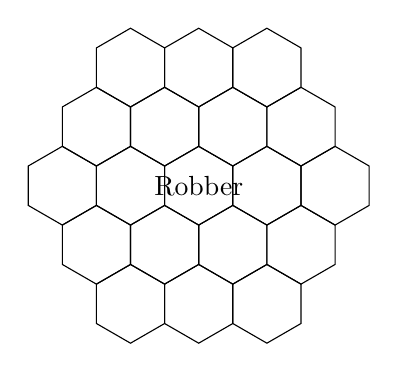
\begin{tikzpicture} [hexa/.style= {shape=regular polygon,regular polygon sides=6,minimum size=1cm, draw,inner sep=0,anchor=south,rotate=30}]
\foreach \j in {0,...,2}{%
\pgfmathsetmacro\end{2+\j} 
  \foreach \i in {0,...,\end}{%
  \node[hexa] (h\i;\j) at ({(\i-\j/2)*sin(60)},{\j*0.75}) {};}  }      
\node [circle,minimum size=1cm] at (h2;2) {Robber};
\foreach \j in {0,...,1}{%
  \pgfmathsetmacro\end{3-\j} 
  \foreach \i in {0,...,\end}{%
  \pgfmathtruncatemacro\k{\j+2}  
  \node[hexa] (h\i;\k) at ({(\i+\j/2-0.5)*sin(60)},{2.25+\j*0.75}) {};}  } 
\end{tikzpicture}
\end{center}

\begin{enumerate}[label=\alph*)]
    \item Is this Markov Chain irreducible? Is it aperiodic? \textbf{Answer - } $\boxed{\textnormal{Yes to both}}$ The Markov Chain is irreducible because it can get from anywhere to anywhere else. The Markov Chain is also aperiodic because the robber can return back to a square in $2, 3, 4, 5, \dots$ moves. Those numbers have a GCD of 1, so the chain is aperiodic.
    \item What is the stationary distribution of this Markov Chain? \textbf{Answer - }Since this is a random walk on an undirected graph, the stationary distribution is proportional to the degree sequence. The degree for the corner pieces is 3, the degree for the edge pieces is 4, and the degree for the center pieces is 6. To normalize this degree sequence, we divide by its sum. The sum of the degrees is $6(3) + 6(4) + 7(6) = 72$. Thus the stationary probability of being on a corner is $3/84 = 1/28$, on an edge is $4/84 =  1/21$, and in the center is $6/84 = 1/14$.
    \item What fraction of the time will the robber be in the center tile in this game? \textbf{Answer - } From above, $\boxed{1/14}$.
    \item What is the expected amount of moves it will take for the robber to return? \textbf{Answer - } Since this chain is irreducible and aperiodic, to get the expected time to return we can just invert the stationary probability. Thus on average it will take $\boxed{14}$ turns for the robber to return to the center tile.
\end{enumerate}


\section{Problem Solving Strategies} \smallskip \hrule height 2pt \smallskip

Contributions from Jessy Hwang, Yuan Jiang, Yuqi Hou

\begin{enumerate} \itemsep -.25em
\item \textbf{Getting Started.} Start by \emph{defining events} and/or \emph{defining random variables}. (''Let $A$ be the event that I pick the fair coin''; ``Let $X$ be the number of successes.'') Clear notion = clear thinking! Then decide what it is that you're supposed to be finding, in terms of your location (``I want to find $P(X=3|A)$''). Try simple and extreme cases. To make an abstract experiment more concrete, try drawing a picture or making up numbers that could have happened. Pattern recognition: does the structure of the problem resemble something we've seen before.
\item \textbf{Calculating Probability of an Event.} Use combinatorics if the naive definition of probability applies. Look for symmetries or something to condition on, then apply Bayes' rule or LoTP. Is the probability of the complement easier to find?
\item \textbf{Finding the distribution of a random variable.} Check the \emph{support} of the random variable: what values can it take on? Use this to rule out distributions that don't fit. - Is there a \emph{story} for one of the named distributions that fits the problem at hand? - Can you write the random variable as a function of a r.v. with a known distribution, say $Y = g(X)$? Then work directly from the definition of PDF or PMF, expressing $P(Y \leq y)$ or $P(Y = y)$ in terms of events involving $X$ only. - For PDFs, find the CDF first and then differentiate. - If you're trying to find the joint distribution of two \emph{independent} random variables, just multiple their marginal probabilities - Do you need the distribution? If the question only asks for the expected value of $X$, you might be able to find this without knowing the entire distirbution of $X$. See the next item.
\item \textbf{Calculating Expectation.} If it has a named distribution, check out the table of distributions. If its a function of a r.v. with a named distribution, try LotUS. If its a count of something, try breaking it up into indicator random variables. If you can condition on something, consider using Adam's law. Also consider the variance formula.
\item \textbf{Calculating Variance.} Consider independence, named distributions, and LotUS. If it's a count of something, break it up into a sum of indicator random variables. If you can condition on something, consider using Eve's Law.
\item \textbf{Calculating $E(X^2)$} - Do you already know $E(X)$ or $\var(X)$? Remember that $\var(X) = E(X^2) - E(X)^2$.
\item \textbf{Calculating Covariance} If it's a count of something, break it up into a sum of indicator random variables. If you're trying to calculate the covariance between two components of a multinomial distribution, $X_i, X_j$, then the covariance is $-np_ip_j$.
\item If $X$ and $Y$ are i.i.d., have you considered using symmetry? 
\item \textbf{Calculating Probabilities of Orderings of Random Variables} Have you considered looking at order statistics? - Remember any ordering of i.i.d. random variables is equally likely.
\item Is this the birthday problem? Is this a multinomial problem?
\item \textbf{Determining Independence} Use the definition of independence. Think of extreme cases to see if you can find a counterexample.
\item Does something look like Simpson's Paradox? make sure you're looking at 3 events. 
\item \textbf{Find the PDF.} If the question gives you two r.v., where you know the PDF of one r.v. and the other r.v. is a function of the first one, then the problem wants you to use a transformation of variables (Jacobian). You can also find the pdf by differentiating the CDF.
\item \textbf{Do a painful integral.} If your integral looks painful, see if you can write your integral in terms of a PDF (like Gamma or Beta), so that the integral equals 1.
\item \textbf{Before moving on.} Plug in some simple and extreme cases to make sure that your answer makes sense.
\end{enumerate}


\section{Biohazards} \smallskip \hrule height 2pt \smallskip

Section author: Jessy Hwang

\begin{enumerate} \itemsep -.25em
\item \textbf{Don't misuse the native definition of probability}  - When answering ``What is the probability that in a group of 3 people, no two have the same birth month?'', it is \emph{not} correct to treat the people as indistinguishable balls being placed into 12 boxes, since that assumes the list of birth months \{January, January, January\} is just as likely as the list \{January, April, June\}, when the latter is fix times more likely.
\item \textbf{Don't confuse unconditional and conditional probabilities, or go in circles with Baye's Rule} - $P(A|B) = \frac{P(B|A)P(A)}{P(B)}$. It is \emph{not} correct to say ``$P(B) = 1$ because we know that $B$ happened.''; P(B) is the probability \emph{before} we have information about whether \emph{B} happened. It is \emph{not} correct to use $P(A|B)$ in place of $P(A)$ on the right-hand side.
\item \textbf{Don't assume independence without justification} - In the matching problem, the probability that card 1 is a match and card 2 is a match is not $1/n^2$. - The Binomial and Hypergeometric are often confused; the trials are independent in the Binomial story and not independent in the Hypergeometric story due to the lack of replacement.
\item \textbf{Don't confuse random variables, numbers, and events.} - Let $X$ be a r.v. Then $f(X)$ is a r.b. for any function $f$. In particular, $X^2$, $|X|$, $F(X)$, and $I_{X>3}$ are r.v.s. $P(X^2 < X | X \geq 0), E(X), \var(X), $ and $f(E(X))$ are numbers. $X = 2$ and $F(X) \geq -1$ are events. It does not make sense to write $\int_{-\infty}^\infty F(X) dx$ because $F(X)$ is a random variable. It does not make sense to write $P(X)$ because $X$ is not an event.
\item \textbf{A random variable is not the same thing as its distribution} - To get the PDF of $X^2$, you can't just square the PDF of $X$. The right way is to use \hyperref[one variable transformations]{one variable transformations} - To get the PDF of $X + Y$, you can't just add the PDF of $X$ and the PDF of $Y$. The right way is to compute the \hyperref[convolutions]{convolution}.
\item \textbf{$E(g(X))$ does not equal $g(E(X))$ in general.} - See the St. Petersburg paradox for an extreme example. - The right way to find $E(g(X))$ is with \hyperref[lotus]{LotUS}.
\end{enumerate}

\section{Recommended Resources} \smallskip \hrule height 2pt \smallskip

\begin{itemize} \itemsep -.25em
\item Introduction to Probability (\url{http://bit.ly/introprobability})
\item Stat 110 Online (\url{http://stat110.net})
\item Stat 110 Quora Blog (\url{https://stat110.quora.com/})
\item Stat 110 Course Notes (\texttt{\href{http://www.mxawng.com/stuff/notes/stat110.pdf}{mxawng.com/stuff/notes/stat110.pdf}})
\item Quora Probability FAQ (\url{http://bit.ly/probabilityfaq})
\item LaTeX File (\texttt{\href{https://github.com/wzchen/probability_cheatsheet}{github.com/wzchen/probability\_cheatsheet}})
\end{itemize}

\begin{center}\emph{Please share this cheatsheet with friends!} \url{http://wzchen.com/probability-cheatsheet}\end{center}

\end{multicols}



\begin{center}

\section{Distributions}

\renewcommand{\arraystretch}{3}
\begin{tabular}{cccccc}
\textbf{Distribution} & \textbf{PDF and Support} & \textbf{Expected Value}  & \textbf{Variance} & \textbf{MGF}\\
\hline \hline
\shortstack{Bernoulli \\ \Bern($p$)} & \shortstack{$P(X=1) = p$ \\$ P(X=0) = q$} & $p$ & $pq$ & $q + pe^t$ \\
\hline
\shortstack{Binomial \\ \Bin($n, p$)} & \shortstack{$P(X=k) = {n \choose k}p^k(1-p)^{n-k}$  \\ $k \in \{0, 1, 2, \dots n\}$}& $np$ & $npq$ & $(q + pe^t)^n$ \\
\hline
\shortstack{Geometric \\ \Geom($p$)} & \shortstack{$P(X=k) = q^kp$  \\ $k \in \{$0, 1, 2, \dots $\}$}& $q/p$ & $q/p^2$ & $\frac{p}{1-qe^t}, qe^t < 1$\\
\hline
\shortstack{Negative Binom. \\ \NBin($r, p$)} & \shortstack{$P(X=n) = {r + n - 1 \choose r -1}p^rq^n$ \\ $n \in \{$0, 1, 2, \dots $\}$} & $rq/p$ & $rq/p^2$ &  $(\frac{p}{1-qe^t})^r, qe^t < 1$\\
\hline
\shortstack{Hypergeometric \\ \Hypergeometric($w, b, n$)} & \shortstack{$P(X=k) = \sfrac{{w \choose k}{b \choose n-k}}{{w + b \choose n}}$ \\ $k \in \{0, 1, 2, \dots,  n\}$} & $\mu = \frac{nw}{b+w}$ &$\frac{w+b-n}{w+b-1}n\frac{\mu}{n}(1 - \frac{\mu}{n})$& $-$  \\
\hline
\shortstack{Poisson \\ \Pois($\lambda$)} & \shortstack{$P(X=k) = \frac{e^{-\lambda}\lambda^k}{k!}$ \\ $k \in \{$0, 1, 2, \dots $\}$} & $\lambda$ & $\lambda$ & $e^{\lambda(e^t-1)}$ \\
\hline
\hline
\shortstack{Uniform \\ \Unif($a, b$)} & \shortstack{$ f(x) = \frac{1}{b-a}$ \\$ x \in (a, b) $} & $\frac{a+b}{2}$ & $\frac{(b-a)^2}{12}$ &  $\frac{e^{tb}-e^{ta}}{t(b-a)}$\\
\hline
\shortstack{Normal \\ $\N(\mu, \sigma^2)$} & \shortstack{$f(x) = \frac{1}{\sigma \sqrt{2\pi}} e^{-\sfrac{(x - \mu)^2}{(2 \sigma^2)}}$ \\ $x \in (-\infty, \infty)$} & $\mu$  & $\sigma^2$ & $e^{t\mu + \frac{\sigma^2t^2}{2}}$\\
\hline
\shortstack{Exponential \\ $\Expo(\lambda)$} & \shortstack{$f(x) = \lambda e^{-\lambda x}$\\$ x \in (0, \infty)$} & $\sfrac{1}{\lambda}$  & $\sfrac{1}{\lambda^2}$ & $\frac{\lambda}{\lambda - t}, t < \lambda$\\
\hline
\shortstack{Gamma \\ $\Gam(a, \lambda)$} & \shortstack{$f(x) = \frac{1}{\Gamma(a)}(\lambda x)^ae^{-\lambda x}\frac{1}{x}$\\$ x \in (0, \infty)$} & $\sfrac{a}{\lambda}$  & $\sfrac{a}{\lambda^2}$ & $\left(\frac{\lambda}{\lambda - t}\right)^a, t < \lambda$\\
\hline
\shortstack{Beta \\ \Beta(a, b)} & \shortstack{$f(x) = \frac{\Gamma(a+b)}{\Gamma(a)\Gamma(b)}x^{a-1}(1-x)^{b-1}$\\$x \in (0, 1) $} & $\mu = \frac{a}{a + b}$  & $\frac{\mu(1-\mu)}{(a + b + 1)}$ & $-$\\
\hline
\shortstack{Chi-Squared \\ $\chi_n^2$} & \shortstack{$\frac{1}{2^{n/2}\Gamma(n/2)}x^{n/2 - 1}e^{-x/2}$\\$x \in (0, \infty) $} & $n$  & $2n$ & $(1 - 2t)^{-n/2}, t < 1/2$\\
\hline
\hline
\shortstack{Multivar Uniform \\ A is support} & \shortstack{$f(x) = \frac{1}{|A|}$\\$  x \in A $} & $-$  & $-$ & $-$\\
\hline
\shortstack{Multinomial \\ \Mult$_k(n, \vec{p}$)} & \shortstack{$P(\vec{X} = \vec{n}) = {n \choose n_1\dots n_k}p_1^{n_1}\dots p_k^{n_k}$ \\ $n = n_1 + n_2 + \dots + n_k$} & $n\vec{p}$ & \shortstack{$\var(X_i) = np_i(1-p_i)$ \\ $\cov(X_i, X_j) = -np_ip_j$} & $\left(\sum_{i=1}^k p_ie^{t_i}\right)^n$ \\
\hline
\hline

\end{tabular}

\hskip 1cm
\section{Inequalities}

\renewcommand{\arraystretch}{1}% Tighter


\begin{tabular}{cccc}
\textbf{Cauchy-Schwarz} & \textbf{Markov} & \textbf{Chebychev} & \textbf{Jensen} \\ 
$|E(XY)| \leq \sqrt{E(X^2)E(Y^2)}$ & 
$\displaystyle P(X \geq a) \leq \frac{E|X|}{a}$ &
$\displaystyle P(|X - \mu_X| \geq a) \leq \frac{\sigma^2_X}{a^2}$ &
$g$ convex: $E(g(X)) \geq g(E(X))$ \\ [0ex]
&&& $g$ concave: $E(g(X)) \leq g(E(X))$ \\ 
\end{tabular}
\end{center}



\end{document}